\documentclass[sigconf]{acmart}

\usepackage{booktabs} % For formal tables

\usepackage{subcaption} % For sub figures

\usepackage{hyperref} % For URLs

\usepackage{graphicx} % For cropping images


% TODO:
% 
% 1) Perhaps integrate this per reviewers suggestion: https://www.researchgate.net/publication/323619573_Revolve_A_Versatile_Simulator_for_Online_Robot_Evolution
%
% 2) We should probably discuss the sensor capabilities and task chosen for this paper as making use of ROS/Gazebo library code.  That ties it in well with the new retooled introduction.
%
% 3) Do we have any more text on Evo-ROS or figures?  Probably should change the balance of figures from experiment to Evo-ROS based ones.  
%
% 4) JMM: Any data supporting how long simulations took?  We can probably call out right in experiments that Ardupilot made it very inefficient for us. (This is done in the Case Study Section - JMM)
%
% McKinley Phone Notes:
% Modify intro to include some of the text from the ROSCON paper.  JMM Done
% Focus more on EvoROS rather than the experiments. JMM Done?
% Leave the rest intact as much as possible.  
% Main change, Section 4 - Case Study (Rename to case study to deemphasize the "new experiment" JMM Done
%
% In intro, the case study illustrates the capabilities of Evo-ROS
% Here's a case study emphasizing different aspects of EvoROS.  We take a problem that is of interest in the community and run it in this framework. 
%
% Workflow diagram of how an individual is evaluated.  
%
% Current Limitations: Section 3, add a sentence to forward reference to our removal of Ardupilot.  
%
% Results and Experiments
% Evo-ROS makes it possible to run these in parallel. 
% Commentary about the sensors. 
%
% Intro:
% Abstract: In this paper we introduce Evo-ROS, change to describe.

% Copyright
%\setcopyright{none}
%\setcopyright{acmcopyright}
%\setcopyright{acmlicensed}
\setcopyright{rightsretained}
%\setcopyright{usgov}
%\setcopyright{usgovmixed}
%\setcopyright{cagov}
%\setcopyright{cagovmixed}<




\copyrightyear{2018}
\acmYear{2018}
\setcopyright{acmcopyright}
\acmConference[GECCO '18 Companion]{Genetic and Evolutionary Computation Conference Companion}{July 15--19, 2018}{Kyoto, Japan}
\acmBooktitle{GECCO '18 Companion: Genetic and Evolutionary Computation Conference Companion, July 15--19, 2018, Kyoto, Japan}
\acmPrice{15.00}
\acmDOI{10.1145/3205651.3208269}
\acmISBN{978-1-4503-5764-7/18/07}

% DOI
%\acmDOI{10.1145/nnnnnnn.nnnnnnn}

% ISBN
%\acmISBN{978-x-xxxx-xxxx-x/YY/MM}

%Conference
%\acmConference[GECCO '18]{the Genetic and Evolutionary Computation
%Conference 2018}{July 15--19, 2018}{Kyoto, Japan}
%\acmYear{2018}
%\copyrightyear{2018}

% phil's commands
\newcommand{\newterm}[1]{{\it #1\/}}      % define a new term in italic
\newcommand{\project}{Evo-ROS} 
%\newcommand{\border}{\rule{\columnwidth}{0.01in} \par\noindent \vspace{0.05in}}
%\newcommand{\border}{\rule{\textwidth}{0.01in} } % gives a textwidth line
\newcommand{\pkm}[1]{{\color{red}[{\bf pkm:} {\em #1}~]}}
\newcommand{\jmm}[1]{{\color{blue}[{\bf jmm:} {\em #1}~]}}
\newcommand{\ajc}[1]{{\color{violet}[{\bf ajc:} {\em #1}~]}}
\newcommand{\gas}[1]{{\color{teal}[{\bf gas:} {\em #1}~]}}
\newcommand{\xpkm}[1]{}
\newcommand{\xjmm}[1]{}
\newcommand{\xajc}[1]{}
\newcommand{\xgas}[1]{}

% Use to remove comments.
% \newcommand{\pkm}[1]{}
% \newcommand{\jmm}[1]{}
% \newcommand{\ajc}[1]{}
% \newcommand{\gas}[1]{}

% \newcommand{\myparagraph}[1]{\paragraph{#1}}      % use either close or spaced paragraphs
\newcommand{\myparagraph}[1]{{\bf #1}}      % use either close or spaced paragraphs
% \newcommand{\myparagraph}[1]{{\vspace{0.075in}\noindent}{{\bf #1}}}      % use either close or spaced paragraphs
\newlength{\figwidth}
\setlength{\figwidth}{1.5in}
\newlength{\skinnywidth}
\setlength{\skinnywidth}{5in}
\newcommand{\hl}[1]{#1}



\begin{document}
\title{Evo-ROS: Integrating Evolution and the Robot Operating System}
\author{Glen A. Simon}
\authornote{Glen Simon is the corresponding author.}
\affiliation{%
  \department{Department of Computer Science and Engineering}
  \institution{Michigan State University}
  \city{East Lansing} 
  \state{Michigan}
  \country{USA}
}
\email{simongle@msu.edu}

\author{Jared M. Moore}
\affiliation{%
  \department{School of Computing and Information Systems}
  \institution{Grand Valley State University}
  \city{Grand Rapids} 
  \state{Michigan}
  \country{USA}
}
\email{moorejar@gvsu.edu}

\author{Anthony J. Clark}
\affiliation{%
  \department{Computer Science Department}
  \institution{Missouri State University}
  \city{Springfield} 
  \state{Missouri} 
  \country{USA}
}\email{AnthonyClark@MissouriState.edu}

\author{Philip K. McKinley}
\affiliation{%
  \department{Department of Computer Science and Engineering}
  \institution{Michigan State University}
  \city{East Lansing} 
  \state{Michigan}
  \country{USA}
}
\email{mckinley@cse.msu.edu}


% \author{Author Names and Affiliations Removed for Double-Blind Review}
\affiliation{
  \institution{\ \\ \ }
  \streetaddress{\ \\ \  }
}

\begin{abstract}
In this paper, we describe the Evo-ROS framework, which is intended to help bridge the gap between the evolutionary and traditional robotics communities.  
%
Evo-ROS combines an evolutionary algorithm with individual physics-based evaluations conducted using the Robot Operating System (ROS) and the Gazebo simulation environment.
% 
% \ajc{But doesn't Evo-ROS not include the external evolutionary algorithm?}
%
% In this manner, Evo-ROS can integrate and apply evolutionary search methods
% to a wide variety of platforms and sensor/actuator suites developed by the ROS community.  
%
Our goals in developing Evo-ROS are to (1) provide researchers in evolutionary robotics with access to the extensive support for real-world components and capabilities developed by the ROS community and~(2) 
enable ROS developers, and more broadly robotics researchers, to take advantage of evolutionary search during design and testing. 
%
We describe the details of the Evo-ROS structure and operation, followed by
presentation of a case study using Evo-ROS to optimize placement of sonar sensors on
unmanned ground vehicles that can experience reduced sensing capability due
to component failures and physical damage.
%
The case study provides insights into the current capabilities and identifies areas 
for future enhancements.  
\end{abstract}

%
% The code below should be generated by the tool at
% http://dl.acm.org/ccs.cfm
% Please copy and paste the code instead of the example below. 
%
\begin{CCSXML}
<ccs2012>
<concept>
<concept_id>10010520.10010553.10010554.10010556.10011814</concept_id>
<concept_desc>Computer systems organization~Evolutionary robotics</concept_desc>
<concept_significance>500</concept_significance>
</concept>
</ccs2012>
\end{CCSXML}

\ccsdesc[500]{Computer systems organization~Evolutionary robotics}

\keywords{Evolutionary robotics, autonomous vehicle, sonar, sensor placement, fault tolerance, Robot Operating System, Gazebo, Ardupilot.}


\maketitle

\section{Introduction}
\label{s:intro}


% In contrast, the broader robotics community can address very complex tasks; the robotic systems utilize many sensor modalities to build a coherent understanding of their environment.
% %
% By providing tested models of commercially available hardware, ROS/Gazebo provides a platform to study high-level behaviors while saving developer time during the design phase.  
% %
% Additionally, results have been shown to transfer to real robots, potentially addressing the ``reality-gap'' often encountered in ER~\cite{Koos2010}.  

% In the {\project} project, we have developed an evolutionary framework that integrates ROS-based simulations for robot evaluation.  
% %
% Our current prototype includes ROS, Gazebo, Ardupilot and MAVROS.    
% %
% The primary goals of the project are twofold. 
% %
% First, the framework enables researchers in ER to take advantage ROS and related simulation tools.
% %
% Second, it enables robot developers to employ evolutionary search during the design process.
% \pkm{I went back and pulled in some of the text from our original intro -- I think it still applies even with the 
% retooling to an Evo-ROS paper...}
%%%%%%%%%%%%%%%%%%%%%%%%%%%%%%%%%%%%
Mobile robotic systems are increasingly being deployed in a wide variety of
applications, such as public safety, agriculture, manufacturing, and supply chain. 
%
Traditionally such systems were operated by remote control, however,
advances in machine learning technologies are making it possible to build robots
that are either partially or fully autonomous.  
%
Such systems are often required to operate
in the face of uncertainty:
e.g., noisy communication, poor weather,
unexpected human input, faulty or damaged sensors and actuators.
% and dynamically adapt to, and
% even mitigate, those situations.
To successfully complete tasks despite adverse events and conditions,
systems must adapt to those situations.
%  requires designing systems that a coupling between system control software and 
% the hardware sensors and actuators that might experience partial or total failure.
% Whereas software and control algorithms can switch operating
% modes quite easily, many aspects of the hardware (for example, the placement 
% of sensors) are generally fixed by the time of deployment.
How can we design the physical robot and its control software so that 
it can operate effectively in such environments? 
The solution space for this problem is enormous, making exhaustive search impractical.

% Designing such systems is a challenging endeavor, one that can potentially be complemented by incorporating evolutionary search methods~\cite{Floreano2008}.  
%
The field of evolutionary robotics~(ER)~\cite{Floreano2008} attempts to address this challenging problem
%
by harnessing the open-ended search capabilities of evolutionary algorithms.
% simulation, many solutions can be explored identifying novel behaviors for different platforms~\cite{Cully2013}. 
An artificial genome specifies the robot's control system and possibly aspects of its morphology.
%
Individuals in a population are evaluated with respect to one or more tasks, with the best performing individuals selected to pass their genes to the next generation.
%
Evolutionary approaches have yielded effective controllers and physical designs for a variety of crawling, swimming, and flying robots~\cite{bongard-lipson, Lipson2000}.  
%
Our own research has applied evolutionary algorithms to optimize both morphology and control
in aquatic and terrestrial robots~\cite{Clark.JournalBB.2015,MooreALIFEJournal}.  
%
%Evolving robot behavior and morphology is interesting in its own right, but f
From an
engineering perspective, a major advantage of evolutionary search is the possible discovery of solutions (as well as potential problems) that the engineer might not otherwise have considered.

%%%%%%%%%%%%%%%%%%%%%%%%%%%%%%%%%%%% 
% 
%%%%%%%%%%%%%%%%%%%%%%%%%%%%%%%%%%%% 
Simulation is an essential component of ER, greatly reducing the time to evolve solutions while avoiding possible damage to physical robots.
%
The ER community typically creates one-off simulation environments by selecting from a few different physics 
engines~(e.g., ODE, Bullet, VoxCAD, Simulink, DART) to evaluate a candidate solution.  
%
Environments are sparse, generally featuring the robot and possibly a few obstacles.  
%
Tasks typically comprise locomotion, navigation, and basic problem solving.
%
% For example, Clark et. al.~\cite{Clark.ALIFE.2012} evolved a flexible caudal fin for a robotic fish using evolutionary search coupled with a physics simulation environment. 
%
% The simulator was customized for the specific problem, and would require a large programmer effort to retool for other problems.  
%
Robots themselves contain only a few sensors, most often custom developed for the specific 
experiment being conducted.  
%
Hence, ER tasks are often limited by the scope of the simulation environment and how much time a developer has to code obstacles, sensors, and the platform itself.  
%
Models are not necessarily shareable between developers due to a lack of standardization.  
%
While many research questions can, and have, been answered by simple simulations, 
it becomes difficult to address more complex questions in these environments.  
%%%%%%%%%%%%%%%%%%%%%%%%%%%%%%%%%%%% 

%%%%%%%%%%%%%%%%%%%%%%%%%%%%%%%%%%%%
In contrast, the broader robotics community can address very complicated tasks,
utilizing multiple sensors and actuators to interpret and navigate 
complex and often adverse environments.
% 
The Robot Operating System~(ROS)~\cite{ROS.main} was developed to facilitate reuse of control software 
across projects, and it has gained a large following in recent years.
%
Together with the Gazebo physics simulator~\cite{Gazebo_paper_ref}, these tools provide tested models of commercially available hardware, enabling study of high-level behaviors while saving developer time during the design phase. 
% The Robot Operating System~(ROS)~\cite{ROS.main} was developed to facilitate code reuse across projects.  
%
% Together with the Gazebo physics simulator~\cite{Gazebo.main}, they provide tested models of commercially available sensors and actuators.  
%
% Gazebo supports a wide variety of commercial sensors and actuators, while providing a robust, tested physics simulation environment for a wide variety of robotic platforms. 
%
% ROS/Gazebo thus provides a platform to study high-level behaviors while saving developer time during the design phase.  
%
Our early experiments~\cite{ClarkSSCI2017} demonstrated the potential benefits of integrating ROS/Gazebo with evolutionary search, but the customized nature of the simulation environment illustrated the need for a more
general platform.
%There, the Adabot uses pre-built, tested libraries for PID control, localization, and commercially available sensors.  
%
%Moreover, ROS control software readily transfers to a physical device.  
% Our early experiments using the Adabot platform~\cite{ClarkSSCI2017} highlight some benefits of integrating ROS/Gazebo with evolutionary search.  
%
%There, the Adabot uses pre-built, tested libraries for PID control, localization, and commercially available sensors.  %
% Still, the simulation environment was highly customized to a particular robotic platform,  illustrating  

%%%%%%%%%%%%%%%%%%%%%%%%%%%%%%%%%%%%

\begin{figure*}[!htb]
    \centering
    
    \begin{subfigure}[t]{0.33\textwidth}
        \centering
        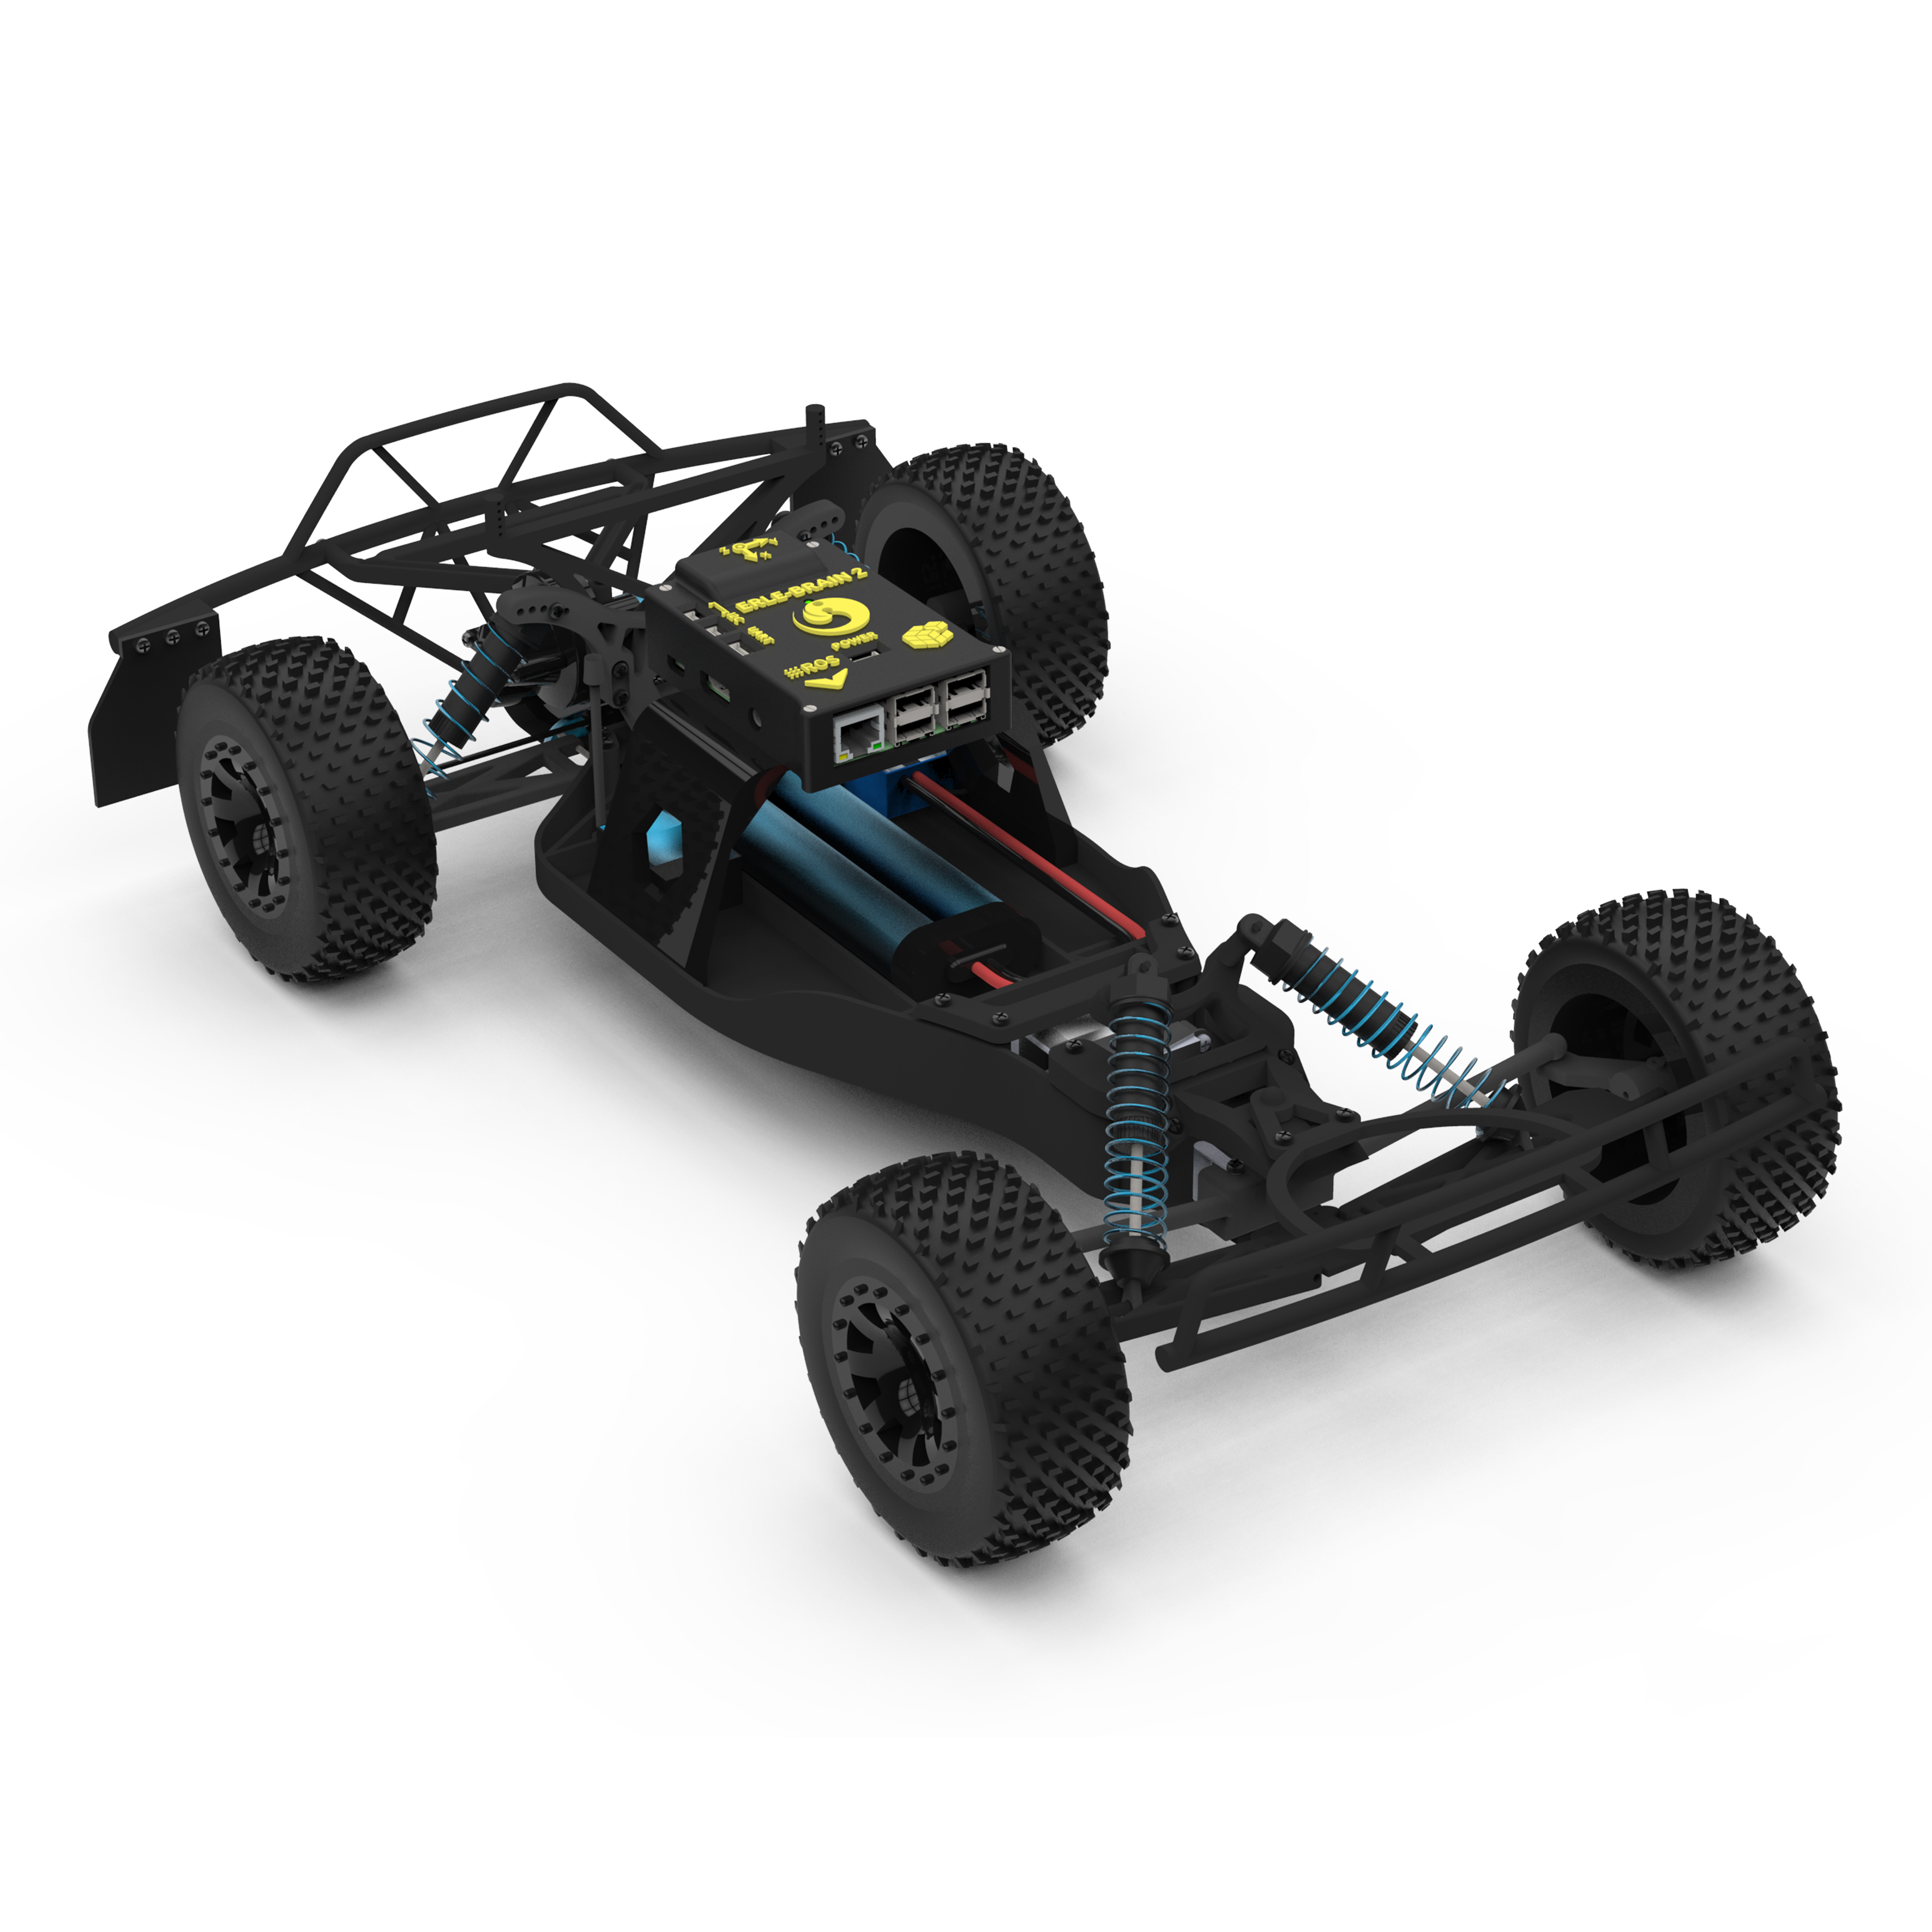
\includegraphics[height=1.2in]{Figures/ErleRover.jpg}
        \caption{Physical Erle-Rover frame}
        \label{real_rover}
    \end{subfigure}%
    ~ 
    \begin{subfigure}[t]{0.33\textwidth}
        \centering
        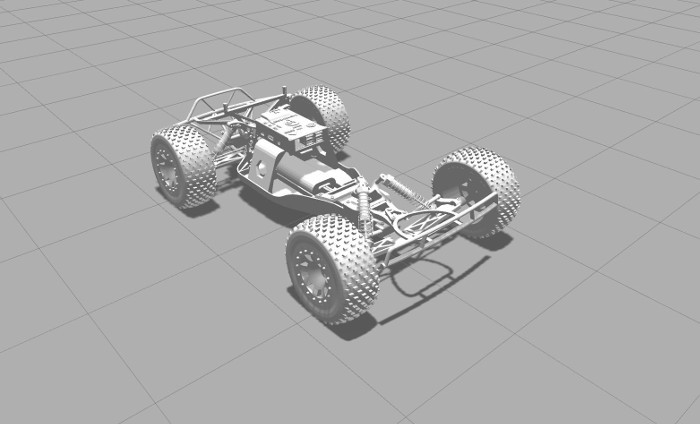
\includegraphics[height=1.2in]{Figures/rover.jpg}
        \caption{Gazebo simulated Erle-Rover}
        \label{sim_rover}
    \end{subfigure}
    ~
     \begin{subfigure}[t]{0.33\textwidth}
        \centering
        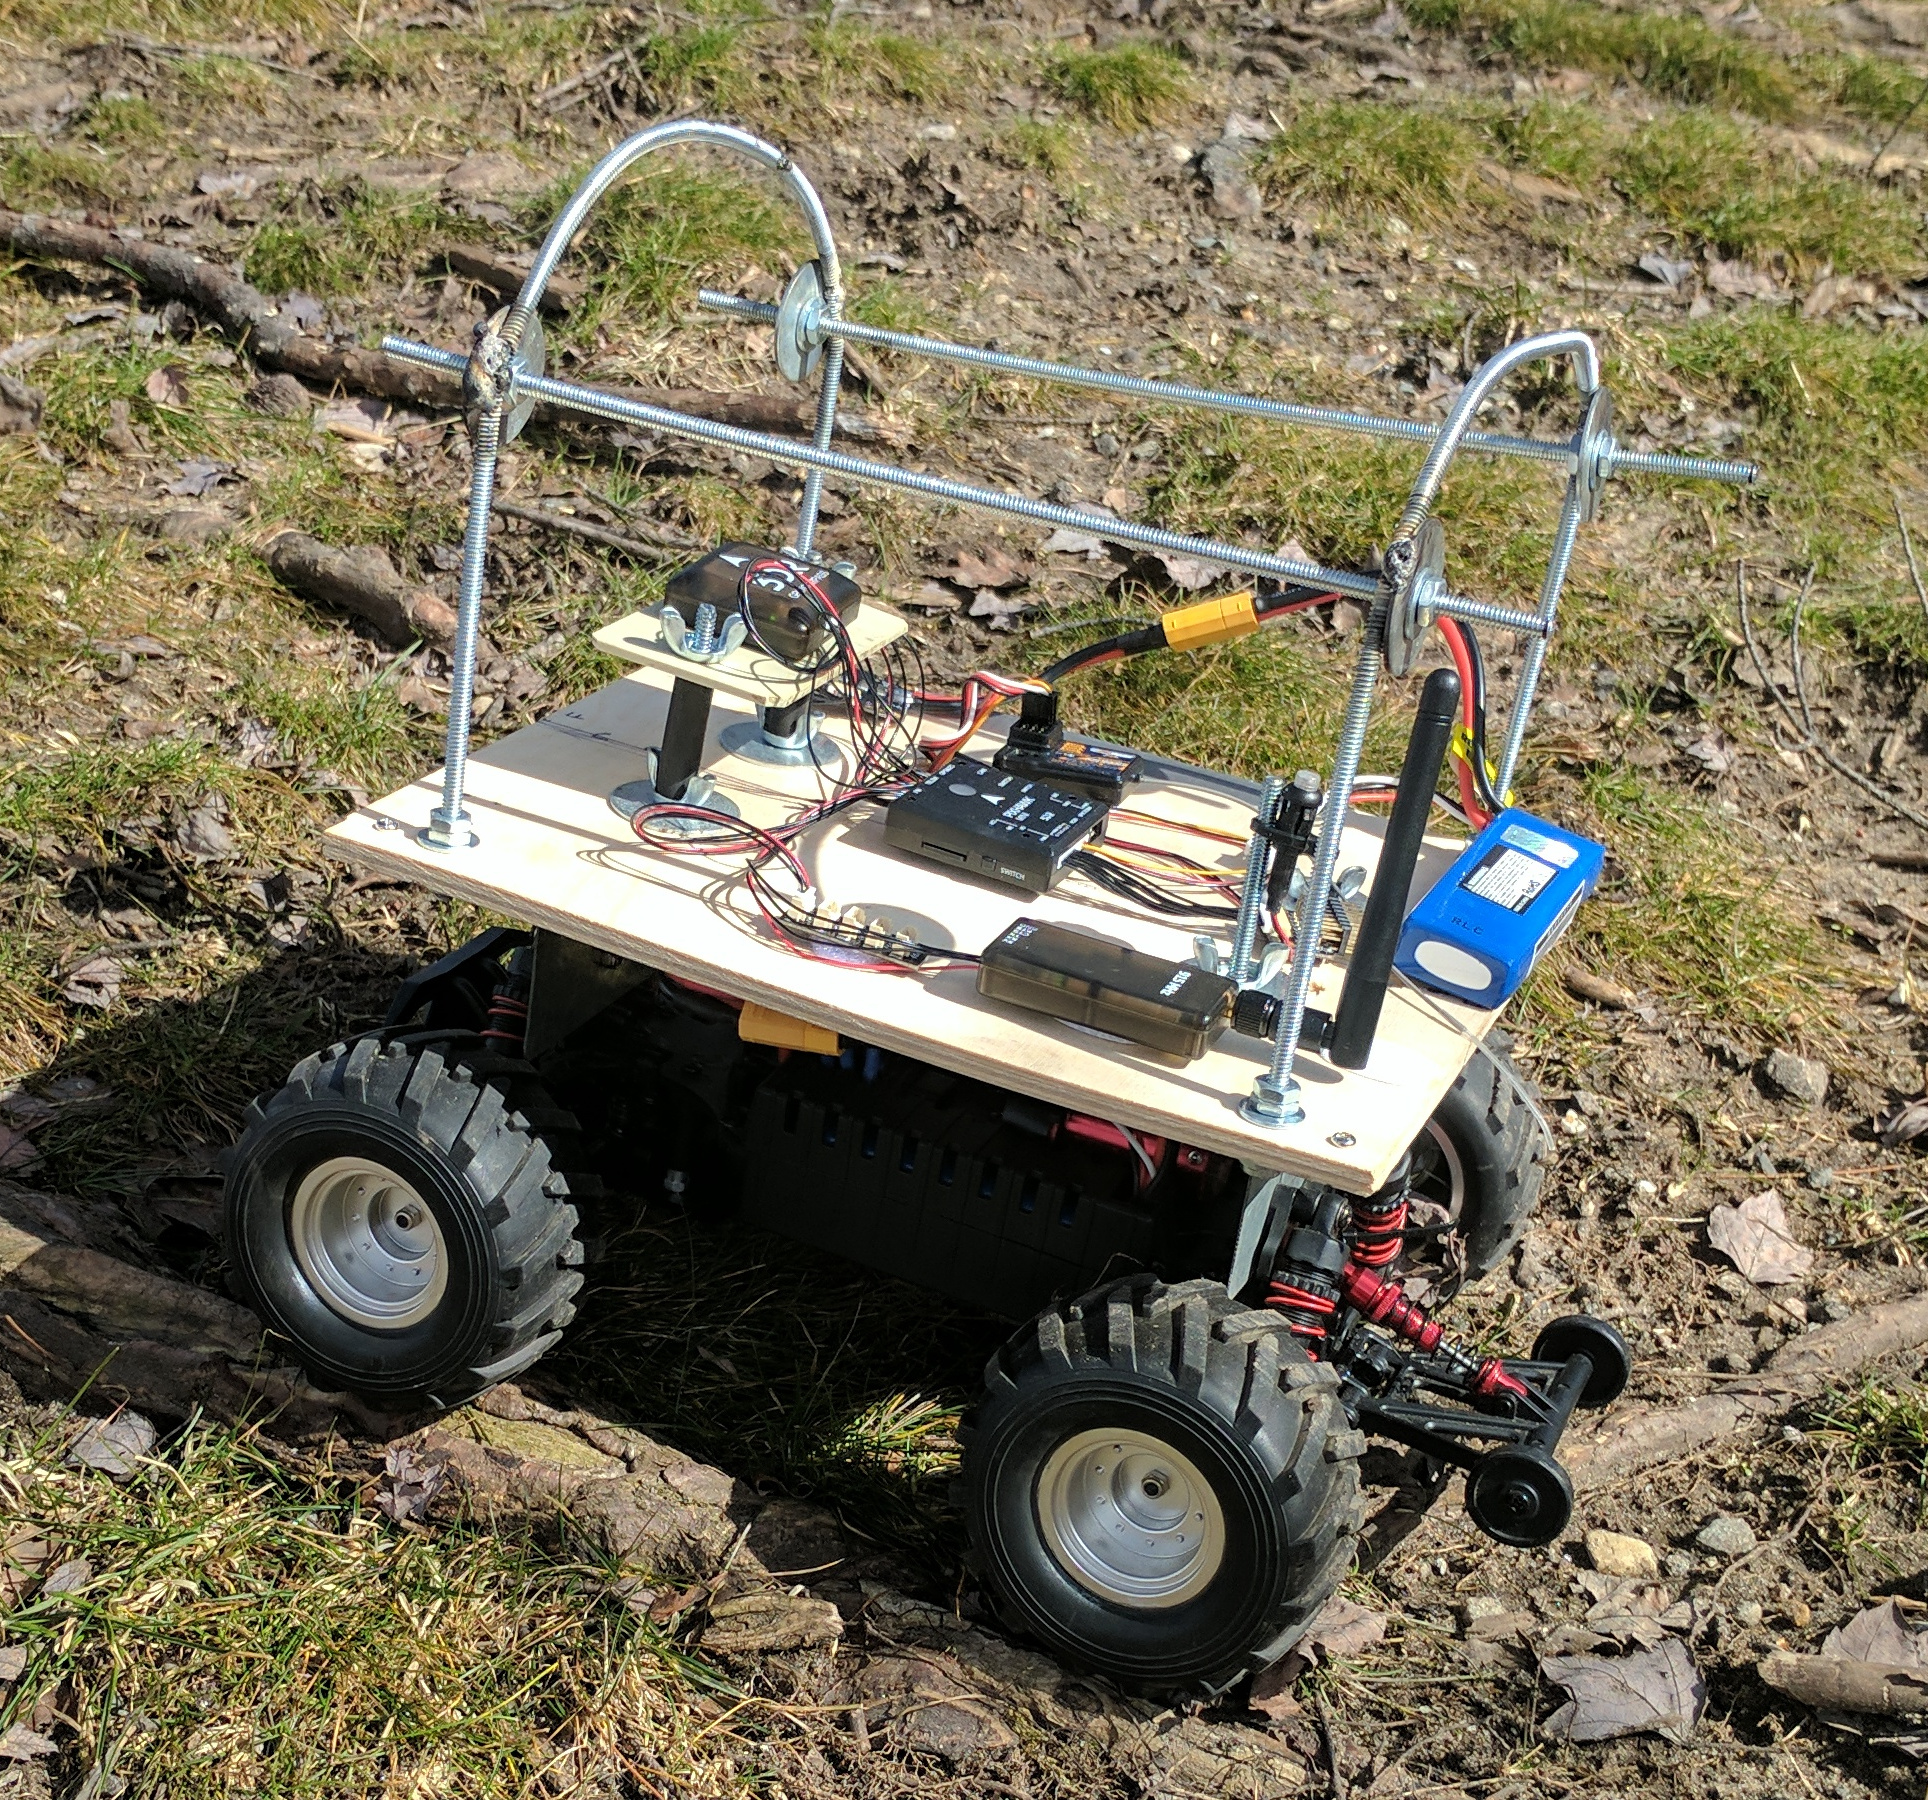
\includegraphics[height=1.2in]{Figures/real_rover_cropped.jpg}
        \caption{Physical rover frame equipped with sensor board, sensors, and a roll cage}
        \vspace{-0.1in}
        \label{msu_rover}
    \end{subfigure}
    \caption{The unmanned ground vehicle platform used in this study.}
    \label{rover_pics}
    \vspace{-0.12in}
\end{figure*}

%%%%%%%%%%%%%%%%%%%%%%%%%%%%%%%%%%%%
The main contribution of this paper is to 
describe Evo-ROS, a software framework integrating evolutionary search, ROS, and Gazebo.  
The current design provides a genetic-algorithm front-end and 
distributes evaluations across many ROS/Gazebo worker instances.  
To our knowledge Evo-ROS is the first ER system that includes simulation tools regularly employed by the broader robotics community.
%
% and available at \url{https://github.com/gsimon2/ros_catkin_ws_src/tree/master/evo_ros}.  
%
%
Evo-ROS internals are described in Section~\ref{s:evoros}. 
Evo-ROS is open-source; a \url{github} link is available at the end of the paper.
%
To demonstrate the operation of Evo-ROS, we conducted a case
study to optimize the 
placement and configuration of sonar sensors on unmanned ground vehicles (UGVs) that may
experience random sensor failures and loss of multiple sensors
due to physical damage.
The target platform is the Erle-Rover~\cite{erle.rover.main}, a commercial terrestrial robot which we 
have tasked with waypoint following under sensor uncertainty. 
%
Figure~\ref{rover_pics} shows the Erle-Rover, its simulation model, and a physical rover equipped with additional sensors. 
Sections~\ref{s:rover} and~\ref{s:results}, respectively, describe the experiments and results of the case study.
%
%Our initial experiment also illuminates areas for ongoing development of the framework, which we discuss later.  
%%%%%%%%%%%%%%%%%%%%%%%%%%%%%%%%%%%%
% 
%%%%%%%%%%%%%%%%%%%%%%%%%%%%%%%%%%%%
% The contributions of this paper are as follows: 
%
% First, we describe the Evo-ROS framework, a software package integrating evolutionary methods with simulation tools regularly employed by the broader robotics community.  
%
%The main To the best of the authors' knowledge, Evo-ROS is the fithis is the first software package to do so.  
%
% Second, we demonstrate the use of Evo-ROS to help design more resilient autonomous systems.  
%
% Specifically, we apply evolution to determine the location of sonar sensors for waypoint following and obstacle avoidance in a commercial unmanned ground vehicle~(UGV), despite random sensor failures and physical damage affecting multiple sensors.  
% 
Finally, in Section~\ref{s:conclusions}, we identify areas for improvement by discussing issues that arose 
during the case study.
%%%%%%%%%%%%%%%%%%%%%%%%%%%%%%%%%%%%
%\vspace{-0.1in}
\section{Background and Related Work}
\label{s:background}
 


% Evolving resilience
% Because it covers a large search space, 
% Evolution is very effective at finding solutions
% beyond preconcptions and therefore 
% bongard, etc.
% -> conclusion?


% sensor placement.
% An importan aspect of resilence is sensing capabiltiy
% Sensor placement is a big issue in robotics

% -> here we exploit that capabilty in placing (sonar)
% sensors on a model of a commercial robot.

\xpkm{PARA 1 (maybe 1\&2): Introduce ER.  Mention/cite works relate to resiliency.  Needs to be 
edited/augmented, as well as smoothed out.}
% Evolutionary robotics (ER)~\cite{Floreano2008} applies principles of biological evolution to the design of robotic systems. 
%
% Individual candidate solutions are evaluated with respect to one or more tasks.  
%
% Evolutionary approaches have produced controllers and physical designs for aquatic, terrestrial, and aerial robots~\cite{bongard-lipson,Lipson2000}.  
%
As with natural evolution, results of many ER studies exhibit a tight coupling between
aspects of morphology, such as sensor positioning, and the controller~\cite{Bongard2015}.
Moreover, the resilience of natural organisms has led researchers to 
apply evolutionary search in order to enhance engineered systems.
Bongard~et~al.~\cite{bongard-lipson} demonstrated the potential of evolution
in {\em self-modeling} terrestrial robots, where the system maintains an internal
``mental image'' of itself and can evolve compensatory behaviors to mitigate damage;
their estimation-exploration algorithm has also been applied to aquatic robots~\cite{Rose.SelfModeling.ERLARS.2013}.
% Model organisms have provided inspiration for aquatic robots~\cite{Clark.ALIFE.2012}, where the flexibility of fins improved performance in a robotic fish.  
% \pkm{Probably mention/cite others.  Maybe our swimming paper?}
Cully~et~al.~\cite{Cully2014} improved and extended this general approach to
enable robots to adapt locomotion strategies in real time, based on sensory feedback.
%


% \paragraph{ER Simulation.}
Despite impressive results from the ER community, however, there remains a disconnect with
the mainstream robotics community, which has also seen major advances in recent years.
\xpkm{cite examples?}
As noted above, ER 
%Simulation is essential to both fields, 
%significantly decreasing the time to 
%evaluate candidate solutions and avoiding damage to a physical platform.
%Within the ER community, 
simulations are typically developed in-house and are simple relative to commercial robots.
% built with tools such as the Open Dynamics Engine~(ODE)~\cite{ODE} and 
% configured per experiment with relatively sparse environments.  
%
% Hence, ER tasks are often limited by the scope of the simulation environment and how much time a developer has to code obstacles, sensors, and the platform itself.  
%
% Moreover, models are not necessarily shareable between developers due to a lack of standardization.  
% 
Silva~et~al.~\cite{Silva.ERissues.2016} recently pointed out these shortcomings and suggested 
possible advantages of adopting tools from mainstream robotics for ER simulations.
In particular, ROS and Gazebo
provide tested models of commercially available actuators and sensors,
saving the ER researcher time in constructing target platforms for evolutionary runs.
Additionally, results have been shown to transfer to real robots, helping
to address the ``reality-gap'' often encountered in ER~\cite{Koos2010}.  
The primary drawback of using high-fidelity simulation in an evolutionary algorithm
is the overhead needed for evaluations.
Our view is that this issue can be partially addressed through 
relatively small-scale parallelization and can eventually be marginalized
with continuing advances in processing capability and larger-scale parallelization.

% \paragraph{Mitigating Sensor Failure}
% \pkm{the GECCO reviewers mentioned other sensor placement studies which we can cite here}
We have realized this approach with the Evo-ROS platform. \xpkm{do we cite the github repository?} \xajc{I suggest we add a placeholder footnote that will eventually link to the github repository but currently is just a comment that the link has been removed to preserve anonymity.}
The particular problem we address in the subsequent case study is optimal placement of sonar sensors
while accounting for possible failures. 
Although these issues are of considerable interest to both the ER and mainstream robotics communities~\cite{Balakrishnan1996,Wang2004,Duckworth.2013.SSRR.Backward}, most studies have focused on fault tolerance and not on sensor placement~\cite{Zhang.2008.FaultTolerance}.
\xpkm{These are pretty old references.  Must be some newer ones from the robotics world.}
% Tony/Jared, can you look for references in this area? See more comments below.}
Evolutionary algorithms are particularly well suited 
to such problems, as they can search large solution spaces, unbiased
by human preconception.
Moreover, evolution can discover ``unlikely-but-possible'' situations that 
might otherwise result in system failure.
\xajc{We should give an example of unlikely-but-possible.}

\xpkm{Any additional transition needed?  Preview results?  Or just leave it and move on to the
details of evoros.}

\xpkm{Should we also comment on any work applying evolution to sensor placement.  
A google search of (robot sensor placement evolution) gives results like these, which I have
not read yet: 
A co-evolution approach to sensor placement and control design for robot obstacle avoidance\\
Evolution of Sensor Placement in Simple Virtual Robots\\
Evolution of Engineering and Information Systems and Their Applications\\
but I suspect placement in the presence of failures is relative open in the ER community, 
though probably better covered in mainstream robotics.}

\xjmm{I added one mainstream and one ER reference in the last paragraph.  Many of the articles I found were on related, but not related enough areas like deploying external sensors in the environment, not on the robot itself.  Perhaps I'm looking under the wrong terms?}

% \pkm{Part 1. Basic flow might follow the ROSCON abstract, to wit:\\
% Evolutionary robotics ->\\
% disconnect with real robots ->\\
% brief intro to Evo-ROS (details to follow in next section->\\
% challenges in terms of speed ->\\
% need for parallelization, which we have done ->//
% (bidirectional) advantages of this approach in applying evolution to real robots
% and making evolution available to roboticists.
% }
% 
% \pkm{Part 2. I think we did a little digging on this and did not find much in the ER
% community, but perhaps you guys know of some relevant works.}

% \vspace{-0.1in}
\section{Evo-ROS Framework}
\label{s:evoros}

\xpkm{This section will provide details on the Evo-ROS framework, but (for the double-blind review)
as if it is a tool we pulled off the Internet and installed on our systems.}

\xpkm{Much of the rest of this section can be adapted from Section 2 (Technologies) 
of your term project report,
except for the details of the Erle-rover simulation, which will be discussed in 
Section~\ref{s:rover}.
We should also include a Figure of the interworkings of Evo-ROS.
I like Figure 3 from your report, though we might need}

\begin{comment}
%%%%%%%%%%%%%%%%%%%%%%
This study employs four main software packages: the Robot Operating System (ROS)~\cite{ROS.main}, Gazebo~\cite{Gazebo.main}, Ardupilot~\cite{Ardupilot.main}, and Evo-ROS. 
%
ROS, Gazebo, and Ardupilot emulate the typical software stack used in in commercial robot design and real-world situations. 
%
ROS is a flexible framework for writing robot controllers consisting of tools, libraries, and conventions that simplify the task of creating complex and robust behavior across a wide variety of robotic platforms. 
%
ROS is commonly used in the manufacturing industry and robotics research.  
%
Controllers are capable of operating robots across diverse platforms such as robotic arms, aerial drones, and UGVs. 
%
Here, ROS is used to implement an obstacle avoidance algorithm for the UGV.
%%%%%%%%%%%%%%%%%%%%%%

%%%%%%%%%%%%%%%%%%%%%%
Simulations are conducted using Gazebo, chosen for its support of complex environments, extensive libraries of simulated sensors modeled after commercially available devices, and the strong coupling with ROS. 
%
Furthermore, Gazebo natively supports ROS code, allowing the same control code to be used in simulation or on the physical UGV.
%
% This statement is too strong, unless we have a supporting reference.
%With these capabilities that Gazebo offers, the reality gap between what is observed in simulation and the behavior of a physical system should be minimal.
%%%%%%%%%%%%%%%%%%%%%%

%%%%%%%%%%%%%%%%%%%%%%
Ardupilot is an advanced, full-featured, and reliable open-sourced autopilot software capable of controlling a wide variety of vehicle systems including rovers, airplanes, multi-rotors, helicopters, boats, and submarines. 
%
Ardupilot has built-in algorithms for the waypoint following task examined in this study.  
%%%%%%%%%%%%%%%%%%%%%%

%%%%%%%%%%%%%%%%%%%%%%
Together, ROS, Gazebo, and Ardupilot produce a robust simulation environment that emulates the operating state a physical UGV will encounter.  
%
The simulated rover is exposed to representations of physical environments that a physical UGV would operate in. % 
However, these software packages are traditionally employed in simulations wherein an experimenter manually configures behaviors and configurations of the robot platform.   
%
Such a process is unsuitable for evolutionary search as many simulations need to be conducted in an automated manner.  
%%%%%%%%%%%%%%%%%%%%%%
\end{comment}

The Evo-ROS framework is intended as a bridge between the evolutionary robotics community and the broader field of robotics.  
Evo-ROS integrates evolutionary algorithms with evaluations constructed using
popular software tools: ROS, Gazebo and, for the case study here, Ardupilot.
ROS~\cite{ROS.main} is a publisher/subscriber framework for writing robot control software 
and includes a large collection of libraries realizing
complex interactions among communicating components.
Here, ROS is used to implement an obstacle avoidance algorithm for the UGV.
%%%%%%%%%%%%%%%%%%%%%%
The Gazebo simulator~\cite{Gazebo_paper_ref}
includes models for a wide variety of commercial devices and 
enables the same control code to be used in both simulated and physical robots.
%%%%%%%%%%%%%%%%%%%%%%
Ardupilot~\cite{Ardupilot.main} is an open-source autopilot stack 
capable of controlling terrestrial, aquatic and aerial vehicles.
Ardupilot has built-in algorithms 
for the waypoint following task addressed in this study.  
%%%%%%%%%%%%%%%%%%%%%%

%%%%%%%%%%%%%%%%%%%%%%

Together, ROS, Gazebo, and Ardupilot can produce a simulation
of commercial robots operating in complex physical environments.
% such as those in which 
% simulation
% environment that emulates the operating state a physical UGV will
% encounter.
% 
% %
% 
% The simulated rover is exposed to representations of physical
% environments that a physical UGV would operate in.
% 
However, these software packages are traditionally used 
during robot development to test new designs manually configured by the experimenter.
%
Moreover, they typically simulate the target platform at real-time speed,
often interacting with a user through a remote control interface identical
to that used with the corresponding physical platform.
%
\xgas{Not sure if this is the place to introduce MAVROS}
\xpkm{Agreed.  Let's put it later.}\xgas{MAVROS is a packaged communication driver that enables ROS processes to communicate to various autopilots, including Ardupilot, by converting messages to follow the MAVLink protocol.}
\xjmm{My thought is that MAVROS muddies the water.  It is not necessary to understand the basic control flow.}
% 
Such a process is unsuitable for evolutionary search, where large numbers of 
simulations need to be conducted in an automated manner and, typically, much
faster than real time.

%%%%%%%%%%%%%%%%%%%%%%


\paragraph{Evo-ROS Structure}
%%%%%%%%%%%%%%%%%%%%%%
Evo-ROS
comprises a set of ROS processes capable of spawning, managing, and changing simulations
carried out by the software tools described above.
%
Specifically, Evo-ROS defines the 
interface between an external evolutionary algorithm (a GA in the present study) and the simulation environment,
enabling individuals from the GA population to be evaluated within the ROS/Gazebo/Ardupilot
stack. 
%
A user would need to construct the genome for their specific problem, and integrate with the provided GA code.  
%
In a typical evolutionary run, multiple Evo-ROS instances are executed
in parallel across virtual machines (VMs).
% 
This configuration 
enables the large number of simulations required for a typical evolutionary run.
% Reality gap comments here are again a bit too strong.  I toned it down a bit, unless we have a citation.
% Ultimately, this combination of software aims to a) 
% utilize a robust, high-performance simulation environment typically employed in the robotics community and B) allowing for the evolved controller code to be directly transferred to a physical UGV.
% %%%%%%%%%%%%%%%%%%%%%%

Figure~\ref{evo_ros_diagram} depicts the main components of Evo-ROS and their interaction
for an individual evaluation.
%
The Evo-ROS ``core'' consists of three main components: 
the transporter, software manager, and the simulation manager. 
%
The transporter is responsible for maintaining communication between an instance of Evo-ROS and the external GA via TCP sockets. 
%
The software manager is responsible for spawning and managing the processes within Evo-ROS, including control~(ROS) and simulation~(Gazebo) software. 
%
A user only has to start the software manager process which then instantiates
all the necessary software (ROS, Gazebo, Ardupilot, etc.).
% 
% \ajc{Doesn't the user also need to write and start an external EA?}
%
The simulation manager monitors various aspects of 
an individual Gazebo simulation, as discussed below.  
%
% \gas{added next 3 sentences.}
%
The rover is equipped with a ROS-based navigation controller that includes waypoint following and obstacle avoidance modes as well as a mechanism for triggering transitions between these modes.
%
These modes are covered in detail in Section~\ref{s:rover}.
%
For the case study, commands generated by ROS-based controllers are sent via MAVROS to the Ardupilot software running on the rover.  
%
They are then transmitted over a TCP link to the vehicle using the MAVProxy protocol. 
%
% \jmm{
Note: The Ardupilot and MAVROS components can be easily swapped out for other low-level control libraries.
% }
% \gas{Note1: I am good with added Jared's above note to the text. Note2: If we are just using ROS-based control (like with the autorally) the output of the Rover Nav controller could be directly looped back to Gazebo. Completely cutting out Ardupilot and MAVROS components. Not sure if it is worth mentioning or not}  
% JMM: I don't think we should overcomplicate it.  Might lead the reviewers astray.
%

% for example, termination conditions.
%In the case of the UGV simulations in this study, termination conditions
%include successful completion of the assigned mission, a UGV collision with another object, 
%and reaching the end of the allotted evaluation time.
%%%%%%%%%%%%%%%%%%%%%%
\vspace{-0.1in}
\begin{figure}[ht]
	\centering
    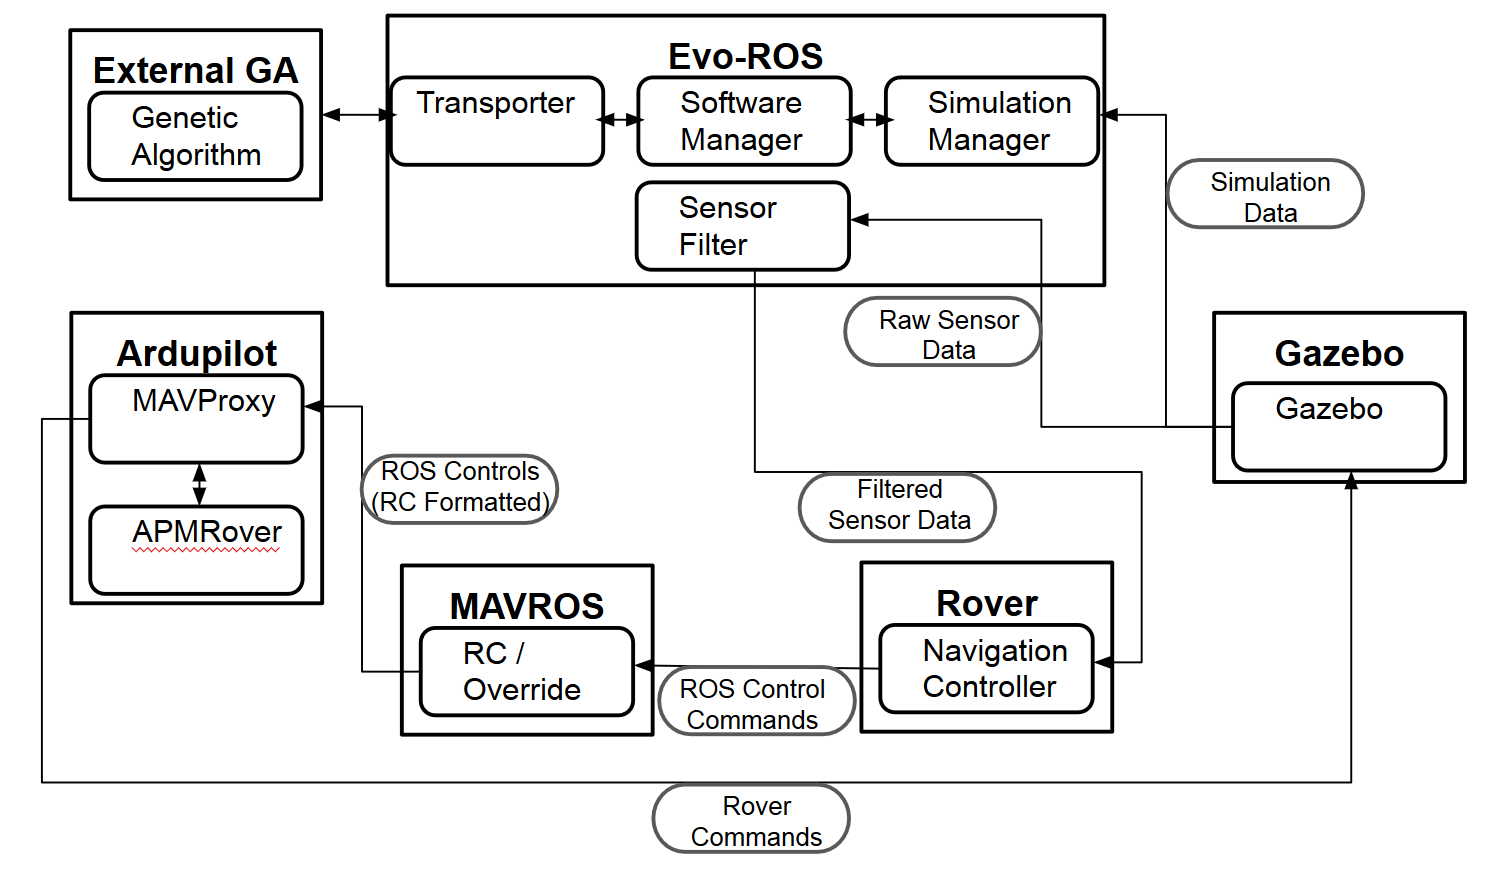
\includegraphics[width=0.47\textwidth]{Figures/evo_ros_diagram.PNG}
    \vspace{-0.05in}
    \caption{Main processes and communication channels 
Evo-ROS management of an individual simulation environment.}
    \label{evo_ros_diagram}
    \vspace{-0.1in}
\end{figure}

%%%%%%%%%%%%%%%%%%%%%%

%%%%%%%%%%%%%%%%%%%%%%

%
%%%%%%%%%%%%%%%%%%%%%%

%%%%%%%%%%%%%%%%%%%%%%
As shown in Figure~\ref{evo_ros_diagram},
an additional component, the sensor filter, has
been added to Evo-ROS for this study.
%
% \jmm{
One of our design goals with Evo-ROS is to allow simple integration of specific components.  The sensor filter is
% }
%
%The sensor filter is a 
a lightweight process that intercepts raw sensor data from Gazebo
and applies filters to the data before forwarding it to the UGV controller. 
%
This filtering could involve injecting noise into sensor readings, introducing delay between when the data is read in Gazebo and delivered to the controller, or selectively neglecting to forward data so that the controller does not receive the readings from specified sensors. Filtering  enables simulating sensor failures in the case study described later.
\xpkm{Hmm, I do not understand what this means.  Further explanation/example?}
\xjmm{I don't think we need this paragraph.  It again muddies the overall message, and how we remove sensor information is not really necessary.  We state that we damage one or more sensors removing it from the pool, and move on.  That has been stated elsewhere.}
%%%%%%%%%%%%%%%%%%%%%%

\begin{figure*}[!htb]
    \centering
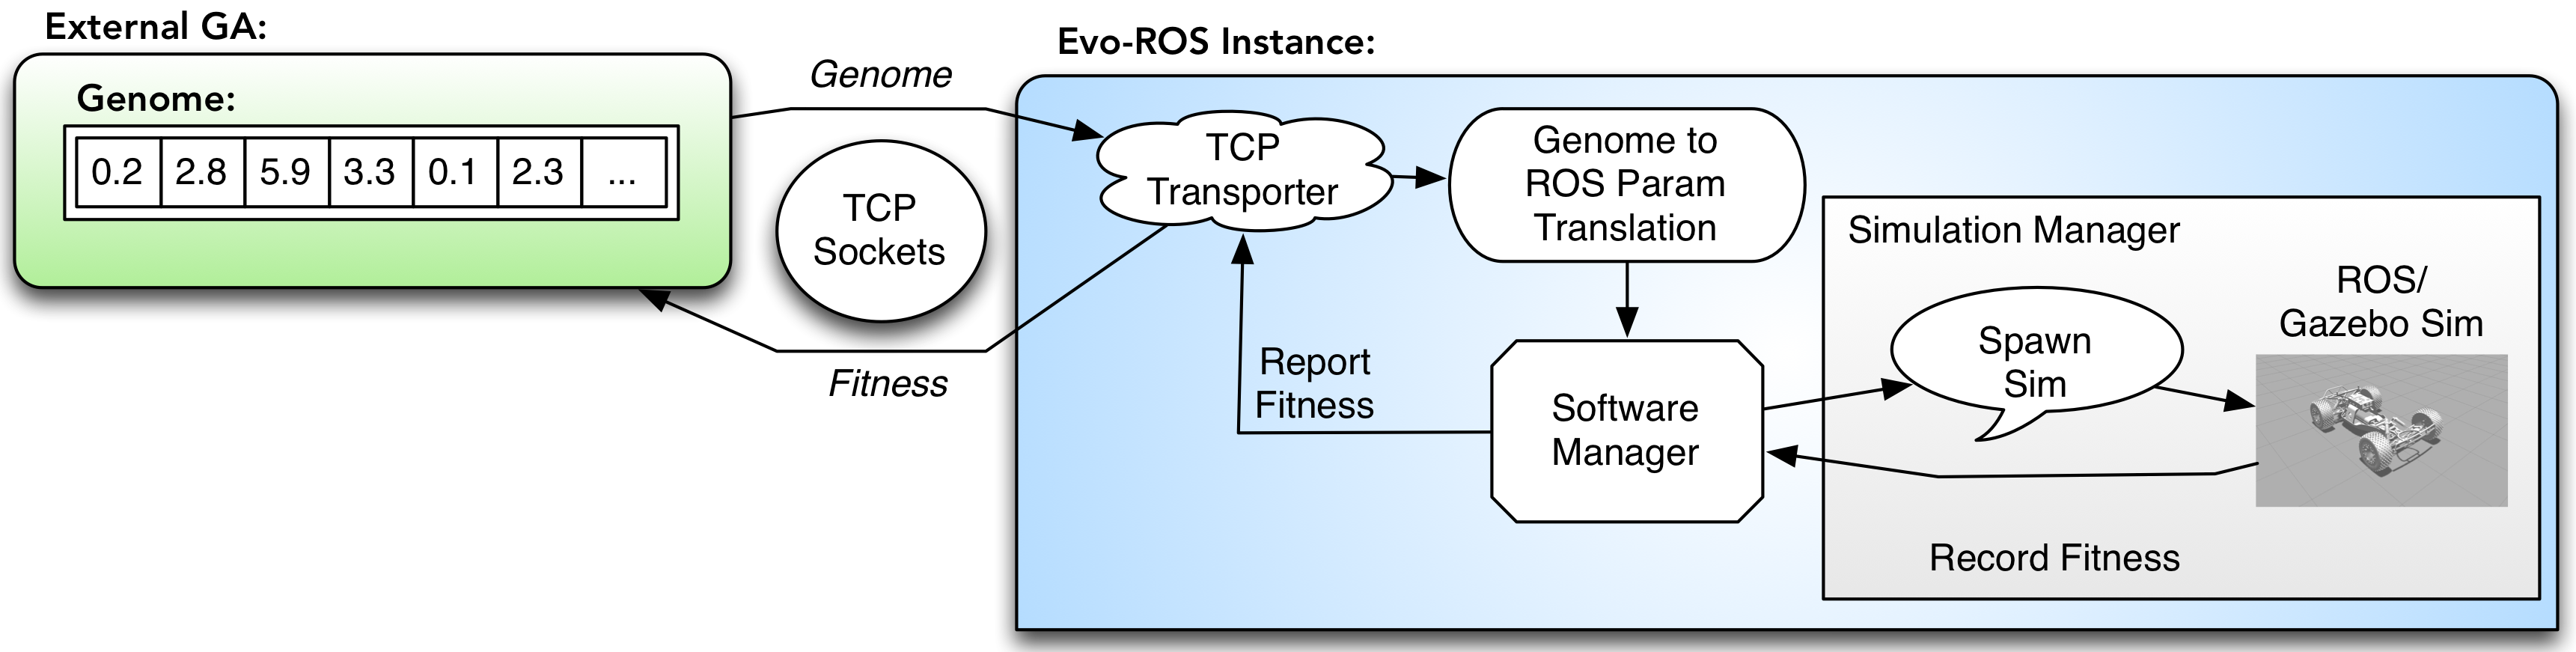
\includegraphics[width=6.25in]{./Figures/Workflow.png}
\vspace{-0.075in}
\caption{The workflow of evaluating an individual genome using an Evo-ROS instance.}
\label{fig:workflow}
\vspace{-0.1in}
\end{figure*}

% \begin{figure}[!htb]
%     \centering
% 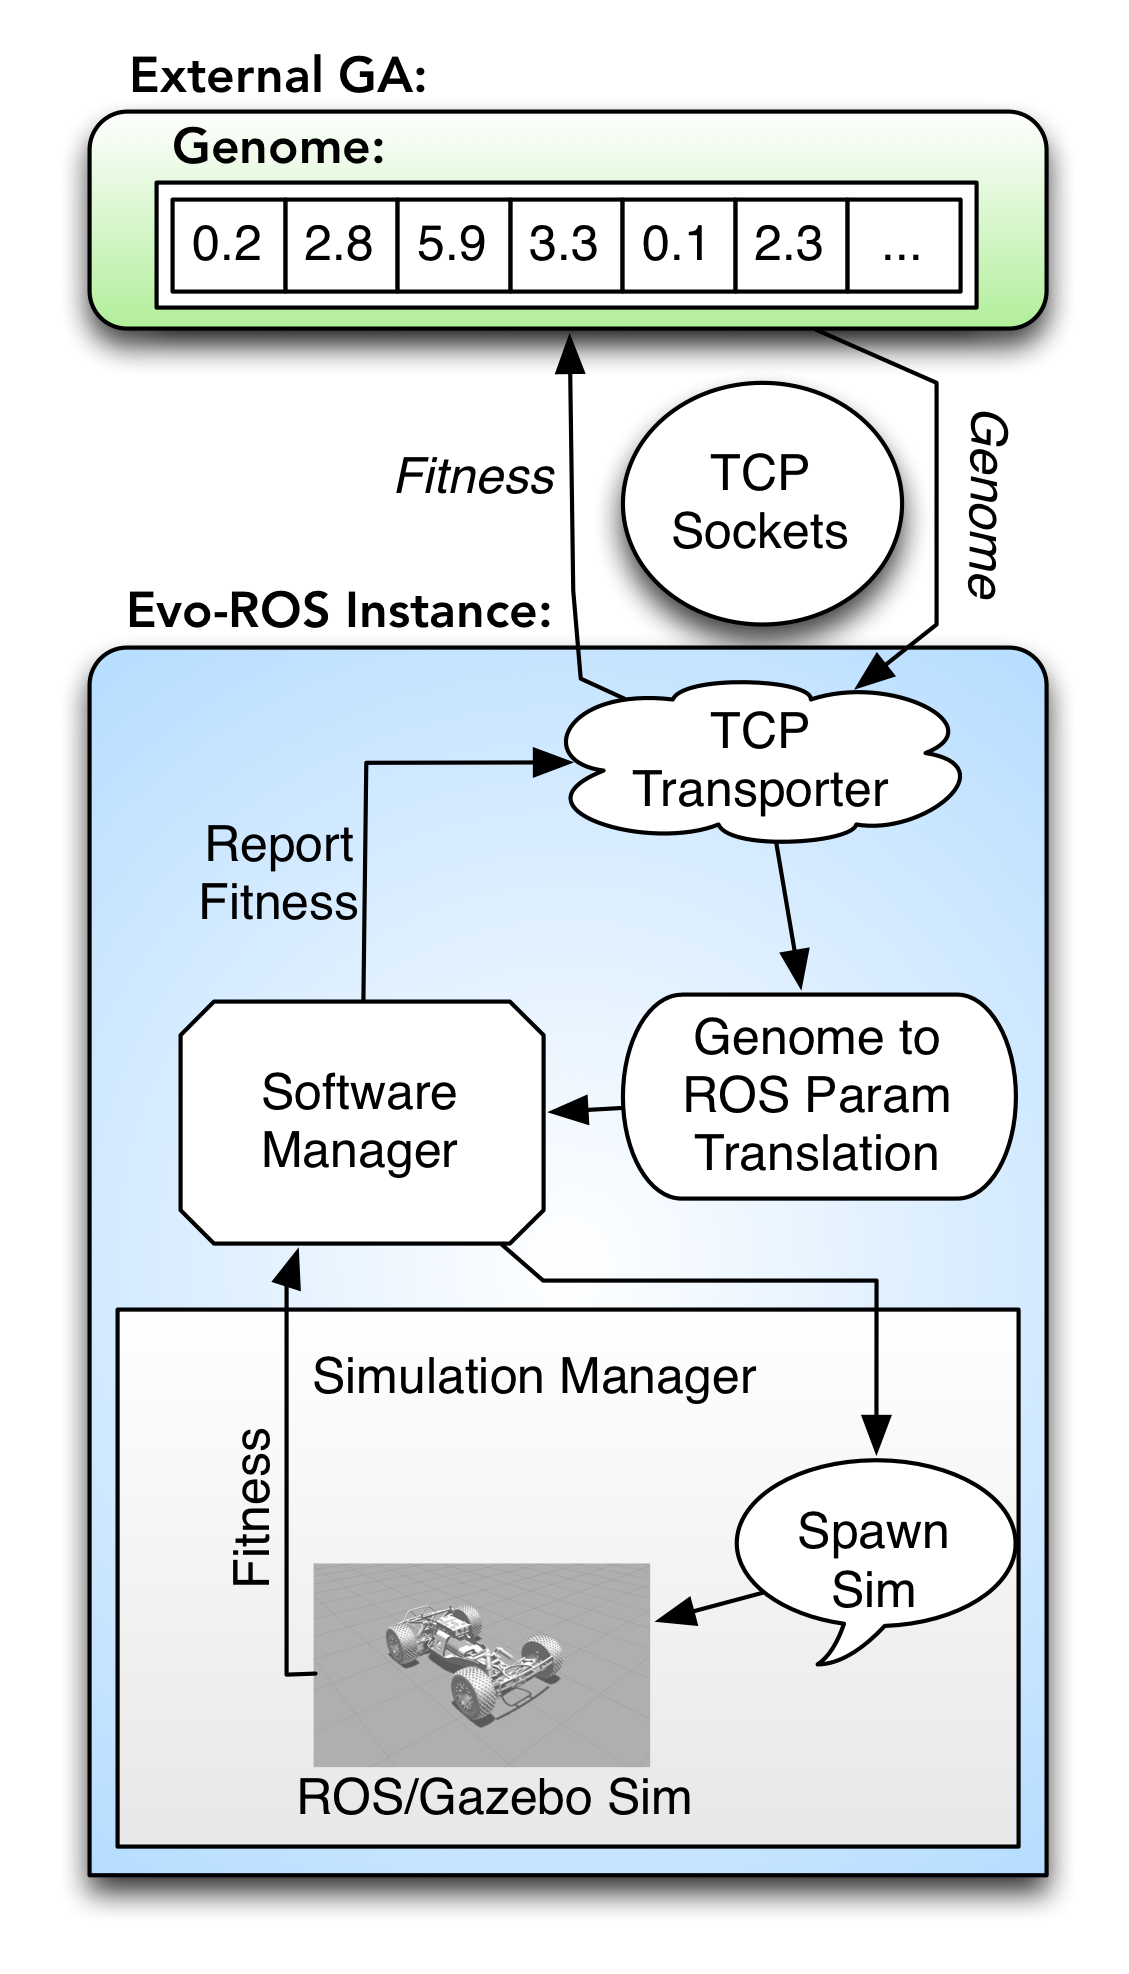
\includegraphics[width=3.5in]{./Figures/Workflow_Sin_Col.png}
% \caption{The workflow of evaluating an individual genome using an Evo-ROS instance.}
% \label{fig:workflow}
% \end{figure}

%%%%%%%%%%%%%%%%%%%%%%
\vspace{-0.1in}
\paragraph{Evo-ROS Workflow}
%
Figure~\ref{fig:workflow} depicts the workflow of evaluating an individual.
% 
First, the GA encodes the attributes of the individual in a genome.
Attributes of an individual could be either behavioral, such as parameter values for various controllers, or physical, such as the number, type, or location of sensors with which this individual is equipped. 
\xpkm{expand on example attributes?}
\xjmm{Wait for the GA section?  Forward reference it?}
%
The genome is transferred via a TCP connection to the transporter process within a single Evo-ROS  instance. 
%
Once received, controller parameters and physical traits from the genome are 
transformed into corresponding ROS parameters.  
%
The transporter then sends a ready flag, via the appropriate ROS topic interface,
to the software manager process. 
%
The software manager determines whether a new simulation environment needs
to be spawned or if the previous one can simply be reset. 
%
(To reduce overhead, 
when evolving controller parameters with unchanging physical traits, the simulation process is persistent and only needs to
be reset before starting a new evaluation.
%
However, when physical traits of the robot are being changed,
such as evolving sensor placements, the software manager
must tear down the simulation environment and modify the robot's
unified robot description format (URDF) model file to reflect the
changes.)
%
The software manager then
spawns the various simulation components, as described above, as well as 
a simulation manager process, and waits for each to initialize.
% simulationThe software manager then spawns all of the software
% applications required for the simulation environment (a ROS
% launch file, a ROS based vehicle controller, Ardupilot, and
% Gazebo), along with 
%
It then hands control to the simulation manager and 
waits until the simulation session completes.

The simulation manager handles an individual evaluation in the physics simulation.  
%
It monitors information within both ROS and Gazebo, including several
metrics describing the state of the simulation.
In this study, such metrics include the speed of travel, 
progression through the mission, distance to each waypoint, collisions with any objects, 
termination conditions (successful completion of the mission, 
reaching the end of the allotted evaluation time).
% as termination conditions.
%
% These could include the UGV colliding with another object, the assigned mission being completed, or if the mission wasn't able to be completed in the alloted amount of time. 
% %
At the conclusion of an evaluation, the simulation manager reports 
the performance of the individual to the software manager. 
%
The software manager forwards the performance report to the transporter, 
which relays it to the GA for calculating fitness.
\xpkm{Figure shows fitness reported by software mgr.  See my email regarding the figure.}
The software manager then cleans up the simulation environment.
This process is repeated for each individual sent to the Evo-ROS instance.
%%%%%%%%%%%%%%%%%%%%%%

%%%%%%%%%%%%%%%%%%%%%%
\paragraph{Current Limitations}
A limiting factor of the Evo-ROS framework using the Ardupilot control framework is the fact that simulations must be capped at near real-time due to the integral 400Hz update loop in the Ardupilot stack.  
%
Furthermore, due to the distributed nature of the ROS system, individual processes within a single ROS instance communicate through a socket-based architecture.  
%
Typically, this means that only a single ROS/Gazebo instance can be run on one physical machine.  
%
We address this issue by creating an individual virtual machine (VM) for each ROS/Gazebo instance and
extend the communication ``fabric'' to include a pool of VMs running on a cluster of
physical nodes.
%
% Therefore, parallelization is required to best utilize computing resources.
%%%%%%%%%%%%%%%%%%%%%%

%%%%%%%%%%%%%%%%%%%%%%
Figure~\ref{evo_multiple} illustrates
our parallelization strategy.
%
Each Evo-ROS instance communicates with the external GA through the transporter process.
%
Instances of Evo-ROS are spawned on multiple VMs spread across several physical machines. 
%
This configuration allows the population of 
the GA to be distributed across many identical simulation environments,
greatly reducing the overall evaluation time per generation.
%
The limiting factor is the number of individual VMs that can be 
spawned across a compute cluster.
%%%%%%%%%%%%%%%%%%%%%%
%\vspace{-0.1in}
\begin{figure}[ht]
	\centering
    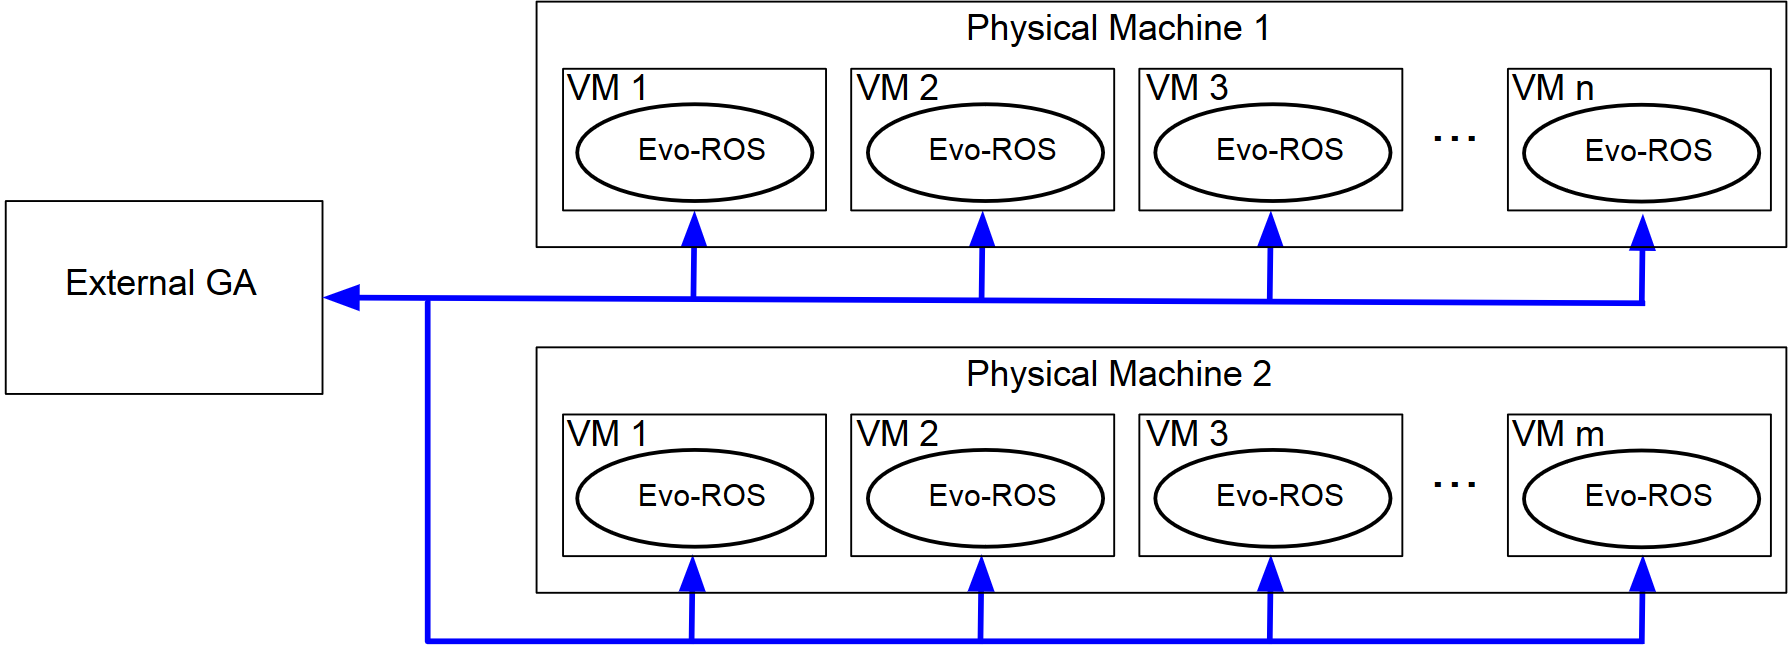
\includegraphics[width=0.45\textwidth]{Figures/evo_ros_distro_setup.PNG}
    \caption{Parallelization of evaluations in Evo-ROS.}
    \label{evo_multiple}
    \vspace{-0.1in}
\end{figure}


\section{Case Study: UGV Sensor Resilience}
\label{s:rover}

\xpkm{This section describes details of the rover, including figures, and discusses
details of its simulation, including sensor operation and the obstacle avoidance control
algorithm. Later, we'll refer back to this algorithm when explaining side placement is likely
due to serpentine motion.}

\xpkm{Do we want to include figure and discussion of the physical rover?
Seeing the connection to real robots usually helps assure the reader that
the study is relevant to the real world.  On the other hand, we don't yet 
have any results of physical experiments.  I suppose we can say that is the
next step of this study?}

%%%%%%%%%%%%%%%%%%%%%%%%%

%\jmm{We next conduct a case study employing a commercially available robot using prebuilt control/sensor algorithms from the ROS/Gazebo Community.  
%
To demonstrate Evo-ROS on a problem of current research interest, we conducted a case study to optimize sensor placement 
on a commercially available UGV using prebuilt control/sensor algorithms from the ROS/Gazebo community.
Figure~\ref{real_rover} shows the target UGV, the Erle-Rover, a car-like robot controlled by ROS~\cite{erle.rover.main}.  
%
Erle Robotics has made available a simulated model of this platform, shown in Figure~\ref{sim_rover}.  
%
The simulated model matches the dimensions and mechanical capabilities of the physical rover, which is
%
% Control is handled through an embedded Linux computer, the Erle-Brain3.
% , that fully supports ROS and ROS 2.0.  
%
% The Erle-Brain3 seamlessly integrates the sensors and power electronics required to perform fully autonomous missions on either ground or aerial vehicles. 
% %
% Physically, the rover 
is 32.5 X 46.5 X 14.5cm with a wheel base of 33.4cm. 
%
As shown in Figure~\ref{msu_rover}, we have augmented our rover with a mounting board to hold
sensors, instruments, and battery packs. To protect the on-board electronics from impact, a roll cage has also been installed. 
%Our future work will involve validating our finding on this physical platform. 
This platform enables the investigation of several 
questions related to resiliency, including optimal sensor placement, discovery of 
execution modes for different conditions, and unwanted feature interaction.
% , and resilience to unfavorable or uncertain conditions. 
%
%We believe that work on such a platform will be directly beneficial to full scale autonomous vehicles.
%%%%%%%%%%%%%%%%%%%%%%%%%

%%%%%%%%%%%%%%%%%%%%%%%%%
%\vspace{-0.1in}
\paragraph{Sensor Placement}
We conducted several preliminary experiments where we allowed the number of sensors and their 
locations to evolve; initially, placement and orientation were not required to be symmetric.
However, we observed little convergence in those runs, and so we enforced symmetry
in all subsequent runs.
Given space limitations, we present a subset of those results here.  
Specifically, all individuals are equipped with
six sonar sensors and symmetry is enforced on the 
their evolved locations and orientations, that is, they evolve as three symmetric pairs.

Figure~\ref{ga_search_space_fig} shows the valid regions of the vehicle where 
sensors can be placed, limited by the 
% Six sensors are placed on the rover with left/right symmetry enforced.  
%
physical configuration of the existing Erle-Rover.
%
Sensors are constrained to the outer 5cm on the front half of the rover.  
%
For this study, the controller does not drive in reverse so we do not consider placement on the rear half of the rover.  
%
Sensor orientation is also constrained to orient sensing regions to the front or sides of the rover.  
Failure models for sensors are described below.
%%%%%%%%%%%%%%%%%%%%%%%%%
\vspace{-0.1in}
\begin{figure}[ht]
	\centering
    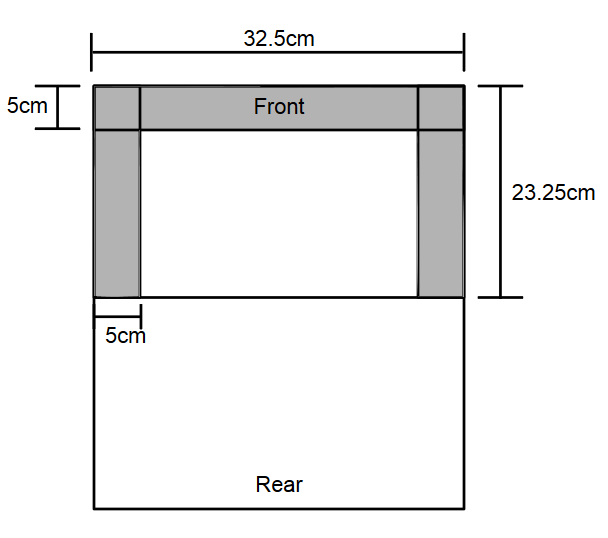
\includegraphics[width=0.32\textwidth]{Figures/sensor_placement_shaded.png}
    \vspace{-0.2in}
    \caption{Sensors can be placed on the outer 5cm on the front half of the robot in the shaded region.}
    \label{ga_search_space_fig}
    \vspace{-0.1in}
\end{figure}

%%%%%%%%%%%%%%%%%%%%%%%%%
\paragraph{Control Hardware}
Rover control is handled through a combination of Ardupilot waypoint navigation and an override when obstacle avoidance is required.  
%
Incorporating Ardupilot requires adding the {\tt arupilot\_sitl\_gazebo\_plugin}~\cite{ardupilot.sitl.plugin} to the simulation environment.  
%
Doing so ensures proper interaction between a Gazebo simulation and the Ardupilot autopilot,
but forces simulations to run at Ardupilot's fixed 400Hz update rate.
%
Evo-ROS implements a step-lock mechanism at each simulation timestep, synchronizing the Gazebo simulation and Ardupilot by pausing the simulation until a new movement command is received.  
%
Evo-ROS then steps the simulation by 2.5ms and returns
new sensor measurements to Ardupilot.
%
Unlike typical Gazebo simulations where the simulator runs without waiting for commands, 
Ardupilot is the master of the simulation clock \cite{erle.simulation}. 
%
The availability of the simulated Erle-Rover model and the Ardupilot plugin provides an accurate representation of the physical rover and portability of evolved controller code between simulated and physical rovers. 
%
% This is helpful when transferring control code while assisting with the reality gap, a topic of our ongoing study.
%
We emphasize, however, that Ardupilot is not integral to Evo-ROS.  As discussed later, we are currently conducting studies that replace Ardupilot with other control software.
% \jmm{From the case study, we have identified removal of the Ardupilot stack as an area for future improvement and discuss further in Section~\ref{s:conclusions}.}
%
%Nonetheless, in future work we plan to create a custom autopilot plugin, freeing us from the 400Hz update limitation imposed by Ardupilot.
%%%%%%%%%%%%%%%%%%%%%%%%%


% \begin{figure*}[!htb]
%     \centering
    
%     \begin{subfigure}[t]{0.33\textwidth}
%         \centering
%         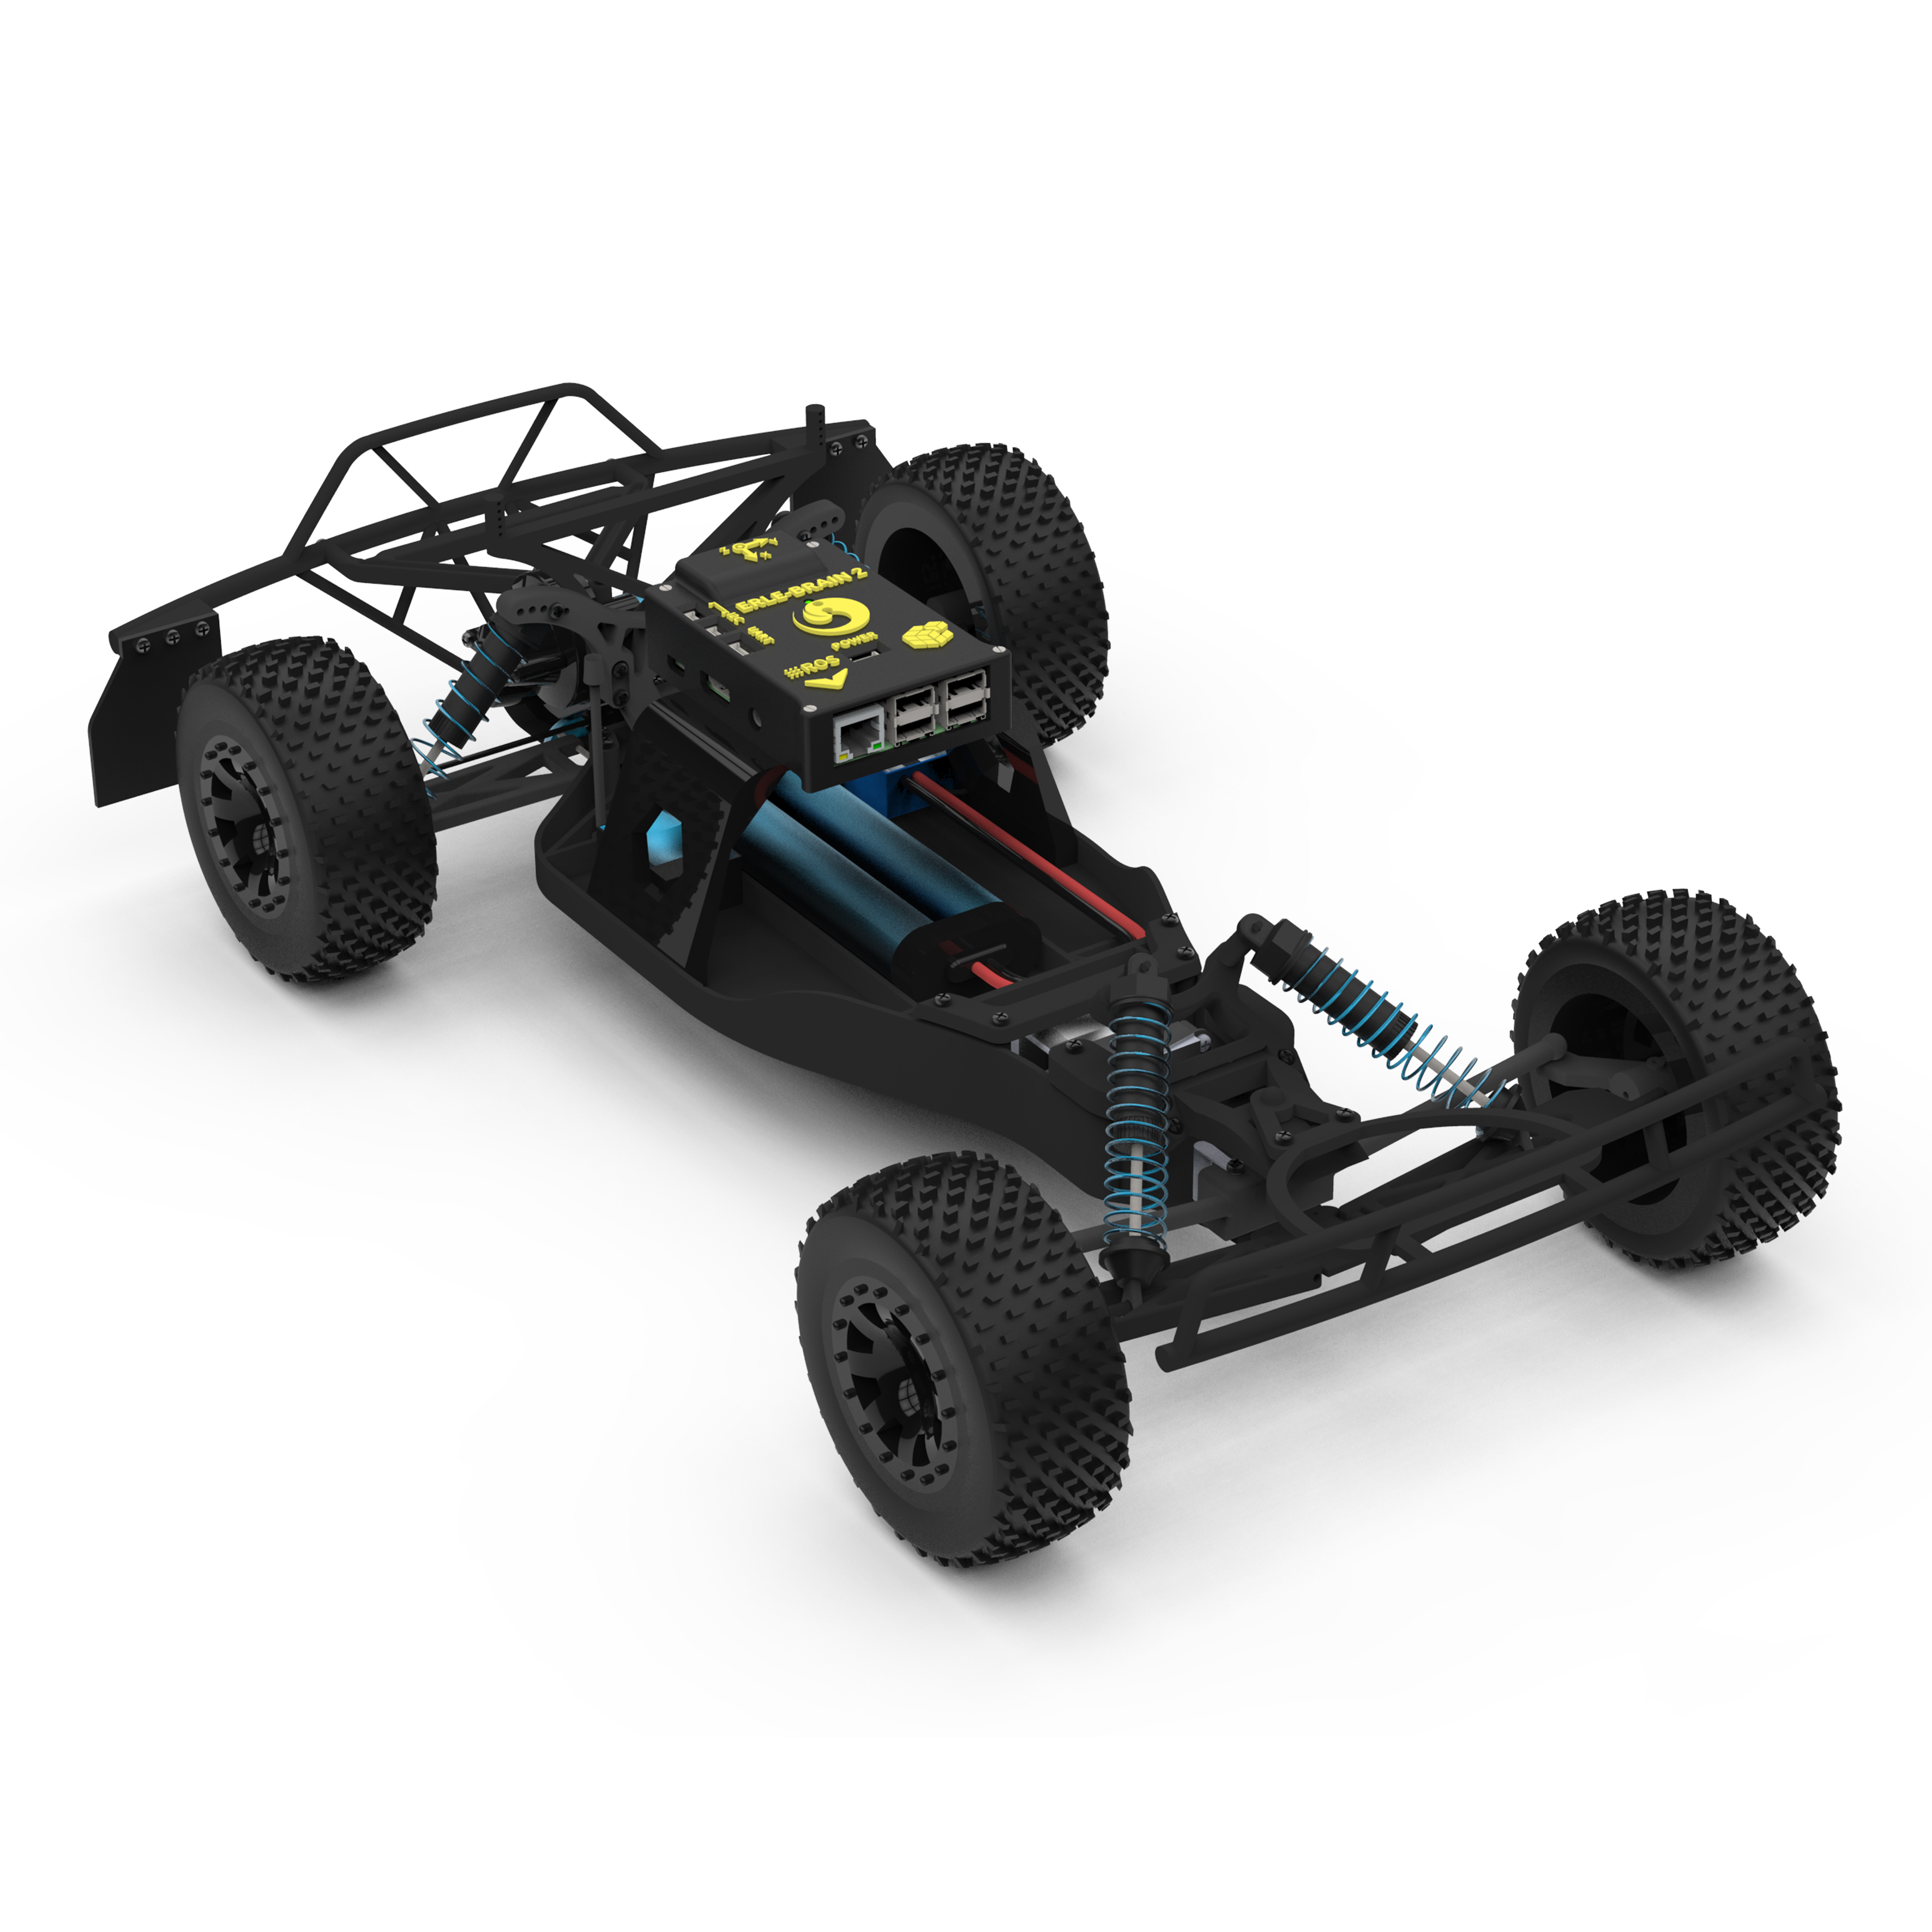
\includegraphics[height=1.2in]{Figures/ErleRover.jpg}
%         \caption{Physical Erle-Rover frame}
%         \label{real_rover}
%     \end{subfigure}%
%     ~ 
%     \begin{subfigure}[t]{0.33\textwidth}
%         \centering
%         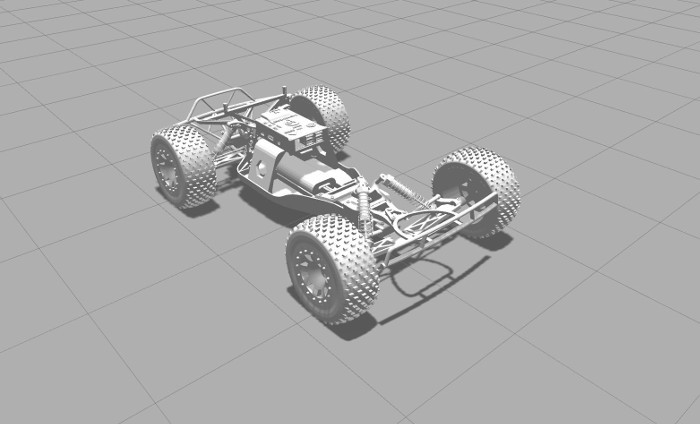
\includegraphics[height=1.2in]{Figures/rover.jpg}
%         \caption{Gazebo simulated Erle-Rover}
%         \label{sim_rover}
%     \end{subfigure}
%     ~
%      \begin{subfigure}[t]{0.33\textwidth}
%         \centering
%         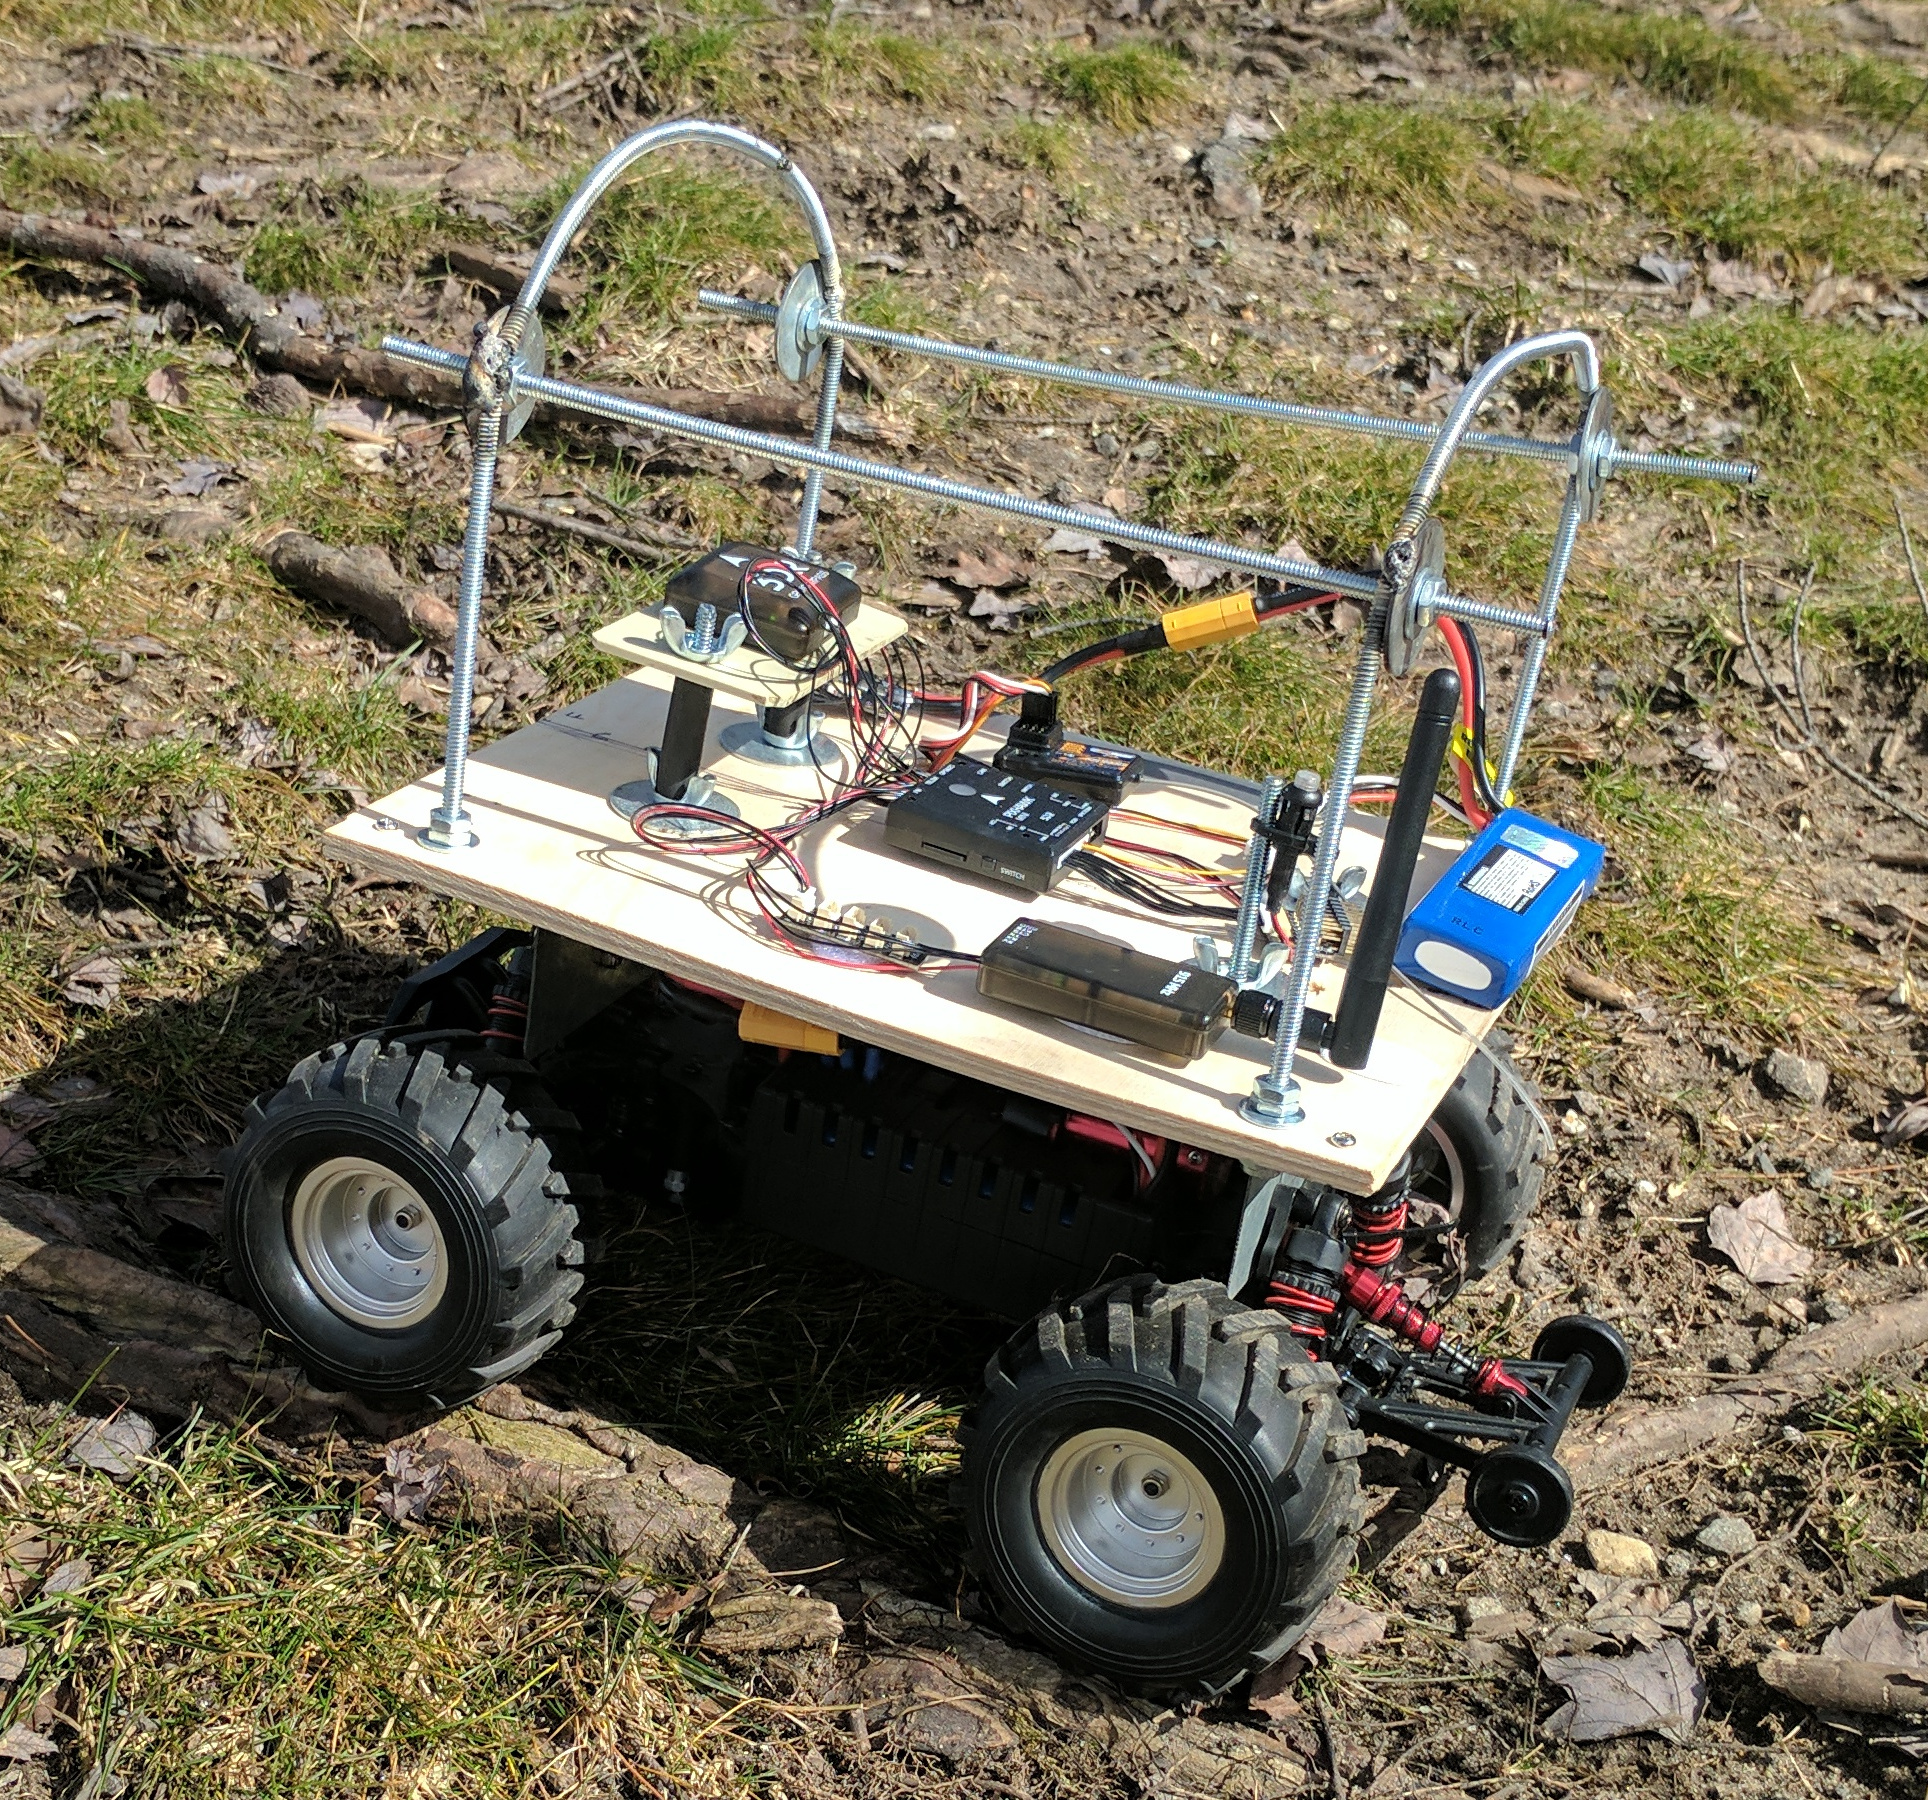
\includegraphics[height=1.2in]{Figures/real_rover_cropped.jpg}
%         \caption{Physical rover frame equipped with sensor board, sensors, and a roll cage}
%         \label{msu_rover}
%     \end{subfigure}
%     \caption{ }
%     \label{rover_pics}
% \end{figure*}

%%%%%%%%%%%%%%%%%%%%%%%%%

\xpkm{Minor point.  Following text mentions mazes.  We need to have introduced that term earlier when
mentioning environments.}

\vspace{-0.08in}
\paragraph{Evaluation}
Figure~\ref{waypoint_mission_fig} depicts one of the three environments
used to evaluate individuals.  
%
% \jmm{
Environments are specified in a Gazebo specific file format, facilitating reuse between experiments.
% }
%
Each rover carries out a pre-defined waypoint following mission, in two phases. 
%
First, a rover navigates through the waypoints within the environment,
eventually returning to the starting location. 
%
If the rover successfully completes the first phase, it then must navigate the waypoints in reverse order, finally returning home again. 
%
Having two phases is intended to avoid
sensor configurations from becoming overfit to missions favoring turns in one direction.
%
In addition, the direction of the first phase
is selected randomly to deter sensor configurations from ``memorizing'' the route. 
%%%%%%%%%%%%%%%%%%%%%%%%%

\vspace{-0.05in}
\begin{figure}[ht]
\centering
    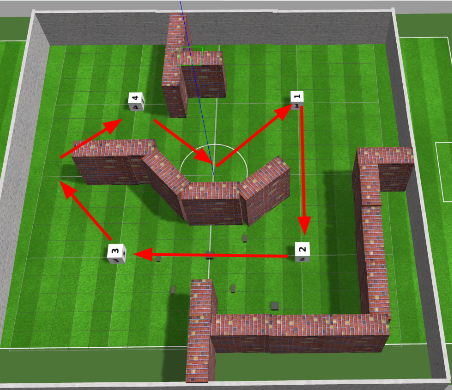
\includegraphics[width=0.4\textwidth]{Figures/waypoint_mission.PNG}
    \vspace{-0.1in}
    \caption{A sample first phase of a mission path consisting of four waypoints in oriented around a home location.}
    \label{waypoint_mission_fig}
    \vspace{-0.1in}
\end{figure}
%%%%%%%%%%%%%%%%%%%%%%%%%

%%%%%%%%%%%%%%%%%%%%%%%%%
\paragraph{Fitness}
Fitness reflects individual performance in three different environments, specifically:
\begin{equation}
fit = \sum_{n=1}^{3} (1 + perc\_complete)^2 + C * (1 + perc\_time\_remaining)^2
\label{eq:fitness}
\end{equation}

\noindent
where $perc\_compelete$ represents the percentage of
mission completed, $C$ is either 1 or 0
indicating whether or not the mission was completed, and
$perc\_time\_remaining$ indicates how much of the allotted
time remained at the completion of the mission.

%%%%%%%%%%%%%%%%%%%%%%%%%

%%%%%%%%%%%%%%%%%%%%%%%%%
%\vspace{-0.1in}
\paragraph{Control}
The control strategy is split into two different modes,~(1) a waypoint following mode
encoded in Ardupilot and~(2) a ROS-based obstacle avoidance mode. 
%
Both modes pass commands to the simulated rover via UDP sockets maintained by Ardupilot. 
%
By default, the waypoint following algorithm
governs navigation when no obstacles are detected by sensors~\cite{Ardupilot.Auto}.
%
% The rover follows a pre-programmed mission script stored in the autopilot composed of navigation commands (i.e., waypoints)
%
Ardupilot navigates between waypoints using a serpentine driving behavior, sweeping the front of the rover through a 60 degree arc as it moves forward, rather than following a straight line. 
%
When at least one sensor detects an obstacle within a threshold distance from the vehicle,
the obstacle avoidance mode preempts the waypoint following algorithm.
%
Obstacle avoidance is
implemented by switching Ardupilot into ``Manual'' mode and sending movement commands from a ROS script.
%
Once the obstacle is cleared, waypoint navigation resumes.  
%%%%%%%%%%%%%%%%%%%%%%%%%

%%%%%%%%%%%%%%%%%%%%%%%%%
\xpkm{This paragraph will be hard for the reader to follow.}
\xjmm{Again, do we need such a technical description?  The previous paragraph explains the two command modes.  I don't know that a reader cares so much about the specific implementation details.  I moved the final sentence of this paragraph to the one above and suggest that we delete the following paragraph.}



The command flow for operating in these two modes can be seen in the bottom half of Figure~\ref{evo_ros_diagram}. In the waypoint following mode, commands are generated by the APMRover process within Ardupilot. In the obstacle avoidance mode, commands are generated by the navigation controller on the rover. These commands are passed through the MAVROS process so that they can be translated to follow the MAVLink protocol. Regardless of the source, the MAVProxy process is responsible for the communication of the commands to either a physical rover or, in our case, a simulated one.
% The bottom half of Figure~\ref{evo_ros_diagram} shows the configuration of 
% these two command modes.
%

%
% Within Ardupilot, waypoint following commands are generated in the 
% % APMRover process and passed to MAVProxy,
%
% which translates these, and override commands, into rover-specific 
% movement commands~(e.g. accelerate, turn). %
% Obstacle avoidance controls are generated in the rover's ROS-based Navigation 
% Controller and passed to a MAVROS process.  
%
% Commands are then sent to MAVProxy along with a command to switch into ``Manual'' mode preempting waypoint navigation for obstacle avoidance.  
%%%%%%%%%%%%%%%%%%%%%%%%%

%%%%%%%%%%%%%%%%%%%%%%%%%
Obstacle avoidance commands are generated using a weighted voting algorithm.  
%
Each sensor that detects an obstacle casts a vote to turn either left or right, depending on the orientation of the sensor. 
%
For example, if a sensor on the front of the vehicle
and angled slightly left detects an obstacle, it would vote to turn right. 
%
Each vote is weighted based on the proximity of the detected object.
%
% A sensor detecting an object two meters away will impact the voting result more than a sensor detecting an object four meters away. 
%
After each sensor has cast its vote, the right and left totals are calculated.
%  along with the difference. 
%
A small difference, with both left and right votes above a certain threshold,
indicates that an object is directly in front of the rover.  
%
The default response is to navigate left around the object. 
%
Otherwise, turning direction is determined by the sign of the difference between the left/right votes, negative indicating a left turn and positive indicating right. 
%
The strength, or sharpness, of the turn is determined by the following equation:
%\vspace{-0.05in}
\begin{equation}
turn\_strength = 1 - \frac{(max\_range - \left | {\sum_{i=0}^{6}w_i * d_i} \right |)}{max\_range}
\label{eq:turn}
%\vspace{-0.05in}
\end{equation}
\noindent
where $max\_range$ is the maximum detection range for the sensor,
$w_i$ is the weight and $d_i$ is the turn direction vote for the $i^{th}$ sensor.  
%
The summation takes into account all voting sensors.
%
%
If $turn\_strength$ is 1.0 the rover will turn as sharply as possible.
%
As $turn\_strength$ approaches 0 the turn becomes more gradual.
%
After an obstacle has been avoided and no sensors report collision threats, 
the autopilot returns to the waypoint following behavior. 
%%%%%%%%%%%%%%%%%%%%%%%%%

%%%%%%%%%%%%%%%%%%%%%%%%%
% \jmm{ TODO: Cut? 
% While the work done in this study focuses on the performance of sensor configurations in a simulated environment, a physical platform, seen in figure \ref{msu_rover}, modeled after the Erle-Rover has been developed and built. This platform rover frame has dimensions of 23.4 x 32.5 x 16cm. Additionally, it is equipped with a mounting board for required sensors, instruments, and battery packs. To protect the on-board electronics from impact, a roll cage has also been installed. Our future work will involve validating our finding on this physical platform. 
% }
%%%%%%%%%%%%%%%%%%%%%%%%%


%\vspace{-0.1in}
\section{Experiments and Results}
\label{s:results}

\xpkm{Sometimes authors describe all the treatments, then describe all the results.
Sometimes that works, but other times it is hard for the reader to keep everything straight.
For this paper, let's take the easier route, which is to introduce each treatment, then
give the results.  I find this "story-telling" approach is easier to follow.}

\xpkm{We need to decide if we are going to include any asymmetric results or not.  If so,
perhaps we can start with a subsection called "Asymmetric Sensor Placement." 
We also note that we let the number of sensors evolve, but did not observe convergence, 
so in the remaining results will fix the number of sensors at 6 and enforce symmetric placement.}

\begin{figure*}[!htb]
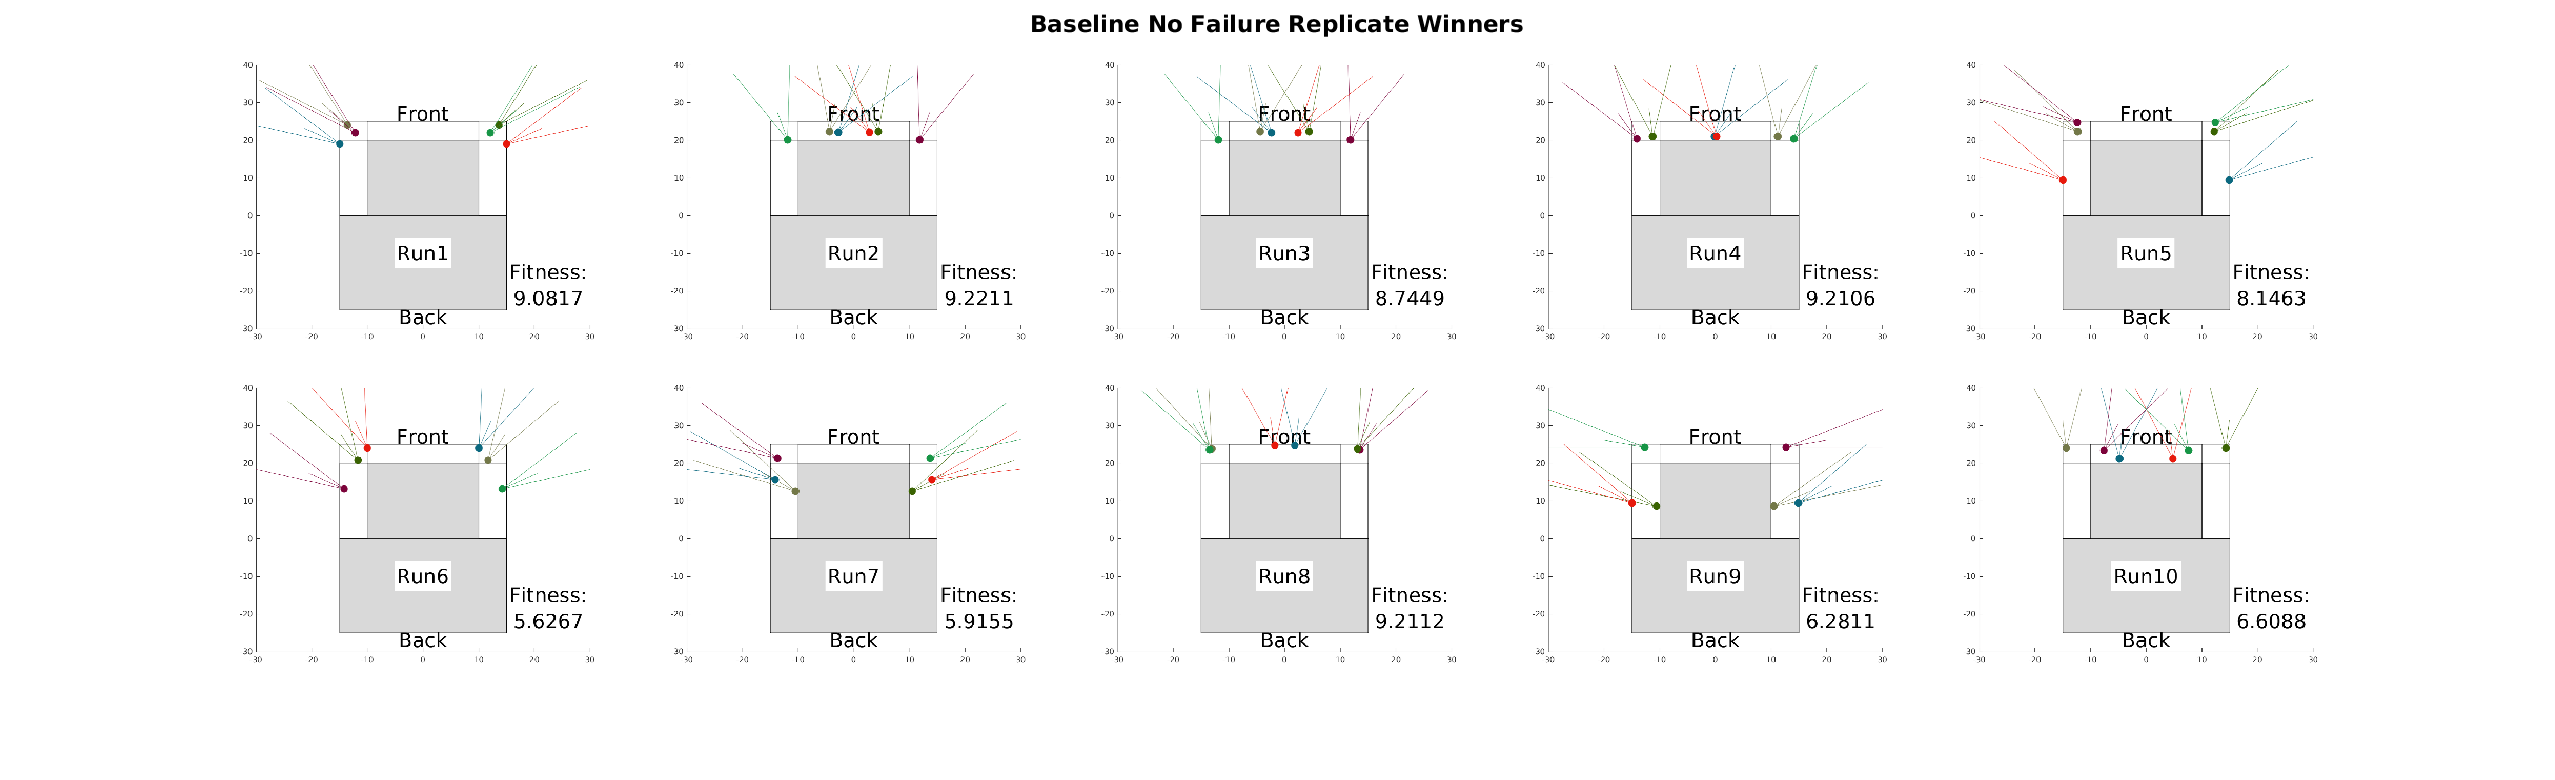
\includegraphics[width=1.0\textwidth]{Figures/6_sonar_symmetric_placement_without_failure_winners_panel_2x5.png}
     \vspace{-0.5in}
%      \includegraphics[width=0.9\textwidth]{Figures/6_sonar_symmetric_placement_without_failure_winners_panel_2X5-crop.pdf}
    \caption{A panel image showing the winning sensor configuration for each replicate in the baseline treatment experiment.}
    \label{baseline_panel_fig}
    \vspace{-0.05in}
\end{figure*}

As noted above, we present only a subset of the results of our experiments, where the
UGV was equipped with six sonar sensors, and left-right symmetry enforced.
We conducted three treatments.
%
First, a greenfield (idealized) scenario establishes a baseline of performance.  
%
%
In this treatment, no sensors fail during the mission and the vehicle
is able to operate under ideal conditions.  
In the next treatment, a single sensor randomly fails during the mission,
simulating a situation where an electrical or mechanical failure arises in the robot.  
%
The final treatment simulates physical damage to the vehicle,
wherein multiple sensors can fail based on their physical proximity to each other.  
We next describe the details of the evolutionary runs, followed by results for each treatment.

%Three different variations of experiments were conducted to evaluate the optimal sensor configuration for six sonar sensors; a greenfield scenario where no sensors fail during the mission, an emulated electrical or mechanical failure scenario where one sensor stops reporting any data partial through the mission mimicking events such as water damage or a broken connection to the sensor, and an impact related failure scenario simulating the rover making a hard collision with an object and incapacitating multiple sensors based on their spatial correlation. 


%%%%%%%%%%%%%%%%%%%%%%%%%
%\vspace{-0.1in}
\paragraph{Evolutionary Parameters}
Table~\ref{GA_param_table} lists the parameters of
the GA used in this study.
%
%
Each individual of the population represents a viable sensor configuration.
% , with the individual's chromosomes containing encodings of multiple sensor locations, relative to the center of the 
% UGV, and orientations.
Specifically, the genome of an individual consists of six behavioral traits relating to six individual sonar sensors. Each of these traits contain four values: a string describing the type of sensor such as 'sonar', the $x$ and $y$ position values of the sensor on the rover as well as a $z$ value that determines the angle at which this sensor should face.
%
After the  population has been evaluated in the simulation environment, tournament selection, with a tournament size of two, creates a parent pool. 
%
Members of the parent pool produce the children pool using crossover with a probability of $0.25$.
%
If crossover does not occur, a child is cloned from a parent.  
%
The original population and the new individuals present in the children pool are combined into the candidate pool, which is larger than the original population size. 
%
A fraction of the members of the candidate pool will randomly undergo mutation,
where the location and/or orientation of one or more sensors can be changed.
%
If mutation or crossover create a new individual, it is marked as unevaluated.  
%
All such individuals are then evaluated via Evo-ROS
before the next generation's population is selected.
%
Elitism is used to maintain the highest performing individual with the rest of the population filled by performing tournament selection.
%%%%%%%%%%%%%%%%%%%%%%%%%
\vspace{-0.1in}
\begin{table}[h!]
    \caption{Genetic Algorithm Parameters.}
    \vspace{-0.15in}
	\centering
    \begin{tabular}{|| c | c ||}
    	\hline
        Population Size & 30 \\
        Generations & 25 \\
        Mutation Probability & 0.15 \\
        Crossover Probability & 0.25 \\
        \hline
    \end{tabular}
    \label{GA_param_table}
%   \vspace{-0.1in}
\end{table}
%%%%%%%%%%%%%%%%%%%%%%%%%

% \begin{figure}[ht]
% 	\centering
%     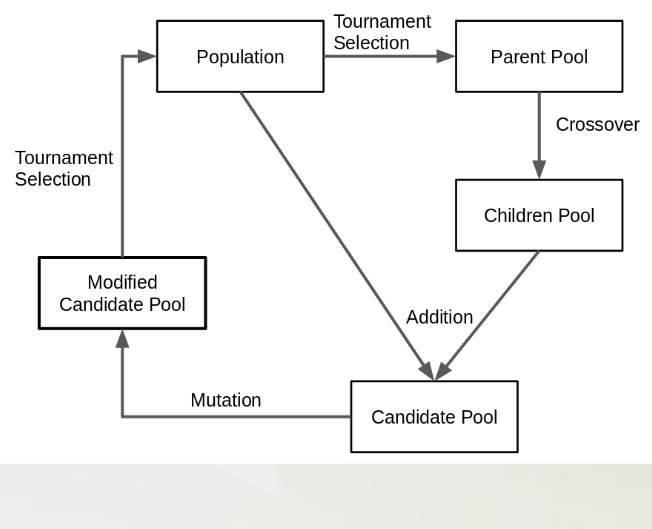
\includegraphics[width=0.4\textwidth, trim={0 1.9cm 0 0}, 		clip]{Figures/GAfigure.PNG}
%     \caption{Model of the GA.}
%     \label{ga_model_fig}
% \end{figure}



% \jmm{TODO: We should move the sensor constraints~(physical location, orientation, symmetry, up to the platform section.

% We are modeling our simulated system after a real rover with hardware already placed on the rover so we must limit the areas in which sonars are placed to the outer 5cm on the front half of the rover. The navigation controller being used never attempts to drive in reverse, so we do not consider the placement of any sensors on the rear half of the rover. The valid areas of sensor placement on the rover are shown in figure \ref{ga_search_space_fig}. We also included some constraints on the orient of the sensor based on the positional coordinates. This pre-engineering does not allow the sensor orients to be faced toward the rear of rover. For this study, the number of sensors is fixed at six and the configurations are required to be symmetric about the y-axis of the rover (left / right symmetry).
% }


% \begin{figure}[ht]
% 	\centering
%     \includegraphics[width=0.4\textwidth]{Figures/rover_sensor_placement_space.PNG}
%     \caption{Sensors can be placed on the outer 5cm on the front half of the robot.}
%     \label{ga_search_space_fig}
% \end{figure}

%Sensor configurations in each experiment were evaluated by equipping them on a simulated rover and allowing the rover to attempt to carry out the mission described in section \ref{s:rover} in three different environments.
% While the mission in each environment remained the same, both the type and the distribution of obstacles that the rover encountered were changed drastically. Between the three environments, the rover was exposed to tall walls, one meter wide cubes, and short cider blocks that had a height just below the height of sensors on the rover. The cider blocks height is important because it makes them insensible at close distances since they are too close to the ground, but visible at distances greater than about half a meter due to the nature of a sonar's conic sensing detecting a wider area the further the distance from the rover. We believe that this invisibility of objects at close distances to the rover will force the rover to choose better paths through clusters of objects, giving a soft distance between each obstacle that it passes rather than approaching it as close as possible without hitting it.  
%  detecting a wider area the further the distance from the rover.  We believe that this invisibility of objects at close distances to the rover will force the rover to choose better paths through clusters of objects, giving a soft distance between each obstacle that it passes rather than approaching it as close as possible without hitting it.

A controller/sensor configuration is evaluated by measuring
the performance of the UGV on waypoint following and obstacle avoidance tasks in 
three different environments, discussed in Section~\ref{s:rover}.   
%
Obstacles in the environments include tall walls, one meter wide cubes, and cinder blocks that are shorter than the height of sensors on the rover. 
%
Cinder blocks thus pose a potential challenge as they are
visible to the rover only at distances greater than 0.5 meters,
due to the cone shaped detection area of a sonar.
%  detecting a wider area the further the distance from the
% rover.
%
We suspect that the cinder blocks will force the vehicle
to evolve navigation strategies
that maintain a distance threshold from obstacles in order
to avoid losing the ability to detect very close objects.

Ten replicates are conducted per experiment. 
%
While this number is considered low for ER experiments, 
the simulation of each mission is computationally expensive 
and is limited to real time due to the use of Ardupilot. 
%
%Ardupilot is built around an inherent 400Hz loop, which limits 
%speed of the Gazebo simulator. 
%
An individual replicate takes between 16 and 24 hours of wall clock time, depending on the average performance of individuals in the replicate.
Attempting to run simulations faster than real-time results in random behavior,
as we cannot assure the control signals are consistent across multiple simulations
of the same controller/sensor configuration. 
%
We plan to address this in future work by replacing the Ardupilot control stack
with a custom autopilot stack, enabling faster than real time simulation. 
%
That said, a goal of this initial case study was to apply evolution to a target system
{\em exactly} matching one from the robotics community, including the use of Ardupilot.


\xpkm{Describe other features of the setup, including the waypoint tasks, fitness calculations, etc.
(note: if we do not include asymmetric runs, the features common to ALL runs can be discussed 
in the introductory material of this section).  
In the following subsections, we will note that the 
treatment is the same as the baseline, except for X, Y, Z.}

%In the baseline treatment, the rover is equipped with six sensors and symmetry is enforced and all sensors work ideally, always reporting on time with accurate data, during the evaluation. This explores the baseline optimal configuration of sensors for a rover. Ten replicates of this baseline treatment were commuted and the winning configurations from each run can be seen in figure \ref{baseline_panel_fig}. An overlay of all of the sensor placements and viewing areas can be seen in figure \ref{baseline_overlay_fig}.

%It can be seen in figure \ref{baseline_panel_fig} that two main patterns appear from this experiment. First, one that is more traditionally accept being an array of sensors placed across the front of the rover with slightly varying angles. This configuration gives the rover a full coverage of the environment directly in front of itself as well as sightly to its sides. The other configuration that emerges is having all of the sensors focus on coverage to the sides of the rover. Well neglecting viewing directly in front of the rover may seem like a weakness, we believe that these configurations are able to thrive because of an artifact of the Ardupilot waypoint navigation behavior. Ardupilot native behavior commonly has the rover drive in a serpentine pattern towards waypoint, causing the front of the rover to swing in an arc up to 60 degrees in magnitude. The driving patterns results in sensors that are mounted facing the side of the rover to detect that are directly in line between the rover's current position and its next waypoint as well as providing extra information to the controller about the environment to the sides of the rover.

%\vspace{-0.1in}
\paragraph{Baseline Experiments}
The UGV is equipped with six sensors and symmetry is enforced across experiments.  
%
In the first treatment, all sensors perform nominally, reporting on time with accurate data.  
%
Figure~\ref{baseline_panel_fig} shows the sensor configuration of best performing
individual in each replicate.  
%
Two main configurations emerge.
%
First is an array of sensors spread across the front of the vehicle,
with slightly varying angles. 
%
This configuration gives the UGV full sonar coverage directly in front, and sightly to its sides. 
%
Second, the sensors ``drift'' toward the sides of the vehicle.
%
Neglecting frontal coverage may seem like a weakness, but it appears that this configuration exploits an artifact of Ardupilot's waypoint navigation behavior. 
%
Specifically, the UGV drives in a serpentine pattern towards each waypoint, causing the orientation of the rover to swing in an arc of up to 60 degrees. 
%
Sensors mounted facing the side of the rover thus sweep through the area in front of the rover, while also providing information to the controller about the peripheral environment.



Figure~\ref{baseline_overlay_fig} overlays the results of the 10 replicates
on a single rover.
%
Common sensing cones and placement are indicated by darker shaded areas.  
%
As seen in Figure~\ref{baseline_panel_fig}, the sensors primarily sweep the forward viewing cone or cover the sides.

\begin{figure}[ht]
	\centering
    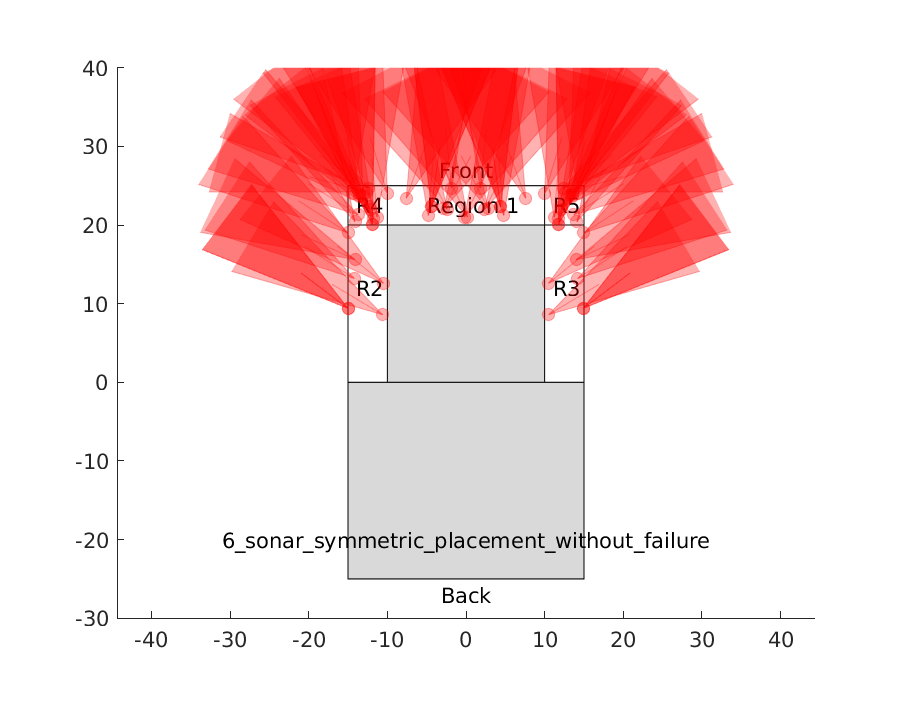
\includegraphics[width=0.5\textwidth]{Figures/6_sonar_symmetric_placement_without_failure_sensor_viewing_area_overlay.png}
    \vspace{-0.45in}
    \caption{Overlay of sensor placements and viewing areas from 10 replicates of the baseline treatment experiment.}
    \label{baseline_overlay_fig}
%    \vspace{-0.1in}
\end{figure}


\xpkm{Need to add a paragraph describing Figure~\ref{evol_track_fig}.
Include or compare with any other plots of evolutionary trajectory?}
A scatter plot of the evolutionary progress of a sample run is shown in Figure~\ref{evol_track_fig}. Here each individual is plotted according to its fitness score and generation. Individuals are color-coded based on their generation, thus individuals from the same generation share the same color. The fitness of the best fit individual and the average fitness for the generation are also plotted. It can be seen that most increases in fitness take place during the first 15 generations, after which fitness plateaus, and the average fitness for each generation approaches that of the most fit individual.
\xjmm{Figure~\ref{evol_track_fig} is currently problematic.  The legend is ambiguous.  It should clearly show best and average, which I assume are the lines on the plot, not the circles.  Perhaps make the best a solid line and the average a dashed line.}

\begin{figure}[ht]
%	\vspace{-0.15in}
	\centering
    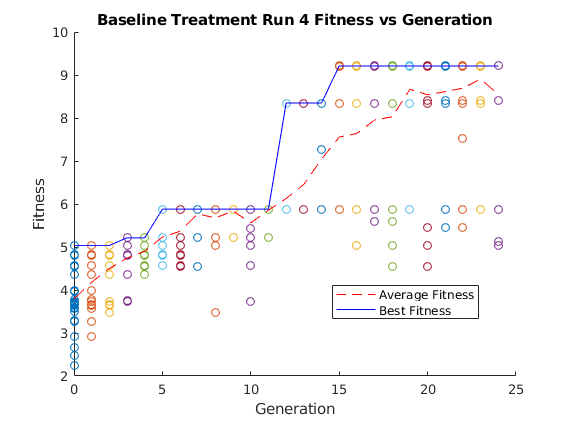
\includegraphics[width=0.45\textwidth]{Figures/fitness_vs_generation_editted.png}
    \caption{Plots of the average and best fitnesses in the population over 25 generations for a sample replicate of the baseline treatment.}
    \label{evol_track_fig}
    \vspace{-0.1in}
\end{figure}

\xpkm{Note treatment same as above but with random failures.
Include specific details of the failure model(s).
Then go on to present results.}

%In the random sensor failure experiment, one random sensor will stop reporting any data at a randomly selected point of time between 40 and 80 seconds into the mission. To put this time into perspective, the rover is allowed 540 seconds to complete the mission with the optimal time being between 360 and 400 seconds depending on the distribution of obstacles in the environment. This means that the failure of a sensor is likely to occur at some point between the first and second waypoint during the first leg of the mission. 

% \vspace{-0.1in}
\paragraph{Random Sensor Failures}
In the second treatment, a randomly
selected sensor fails between 40 and 80 seconds into an individual simulation.
%
The UGV is allowed 540 seconds to complete a mission,
with the optimal time being between 360 and 400 seconds,
depending on the distribution of obstacles. 
%
% Failure of a sensor occurs at some point between the first and second waypoint during the first leg of the simulation. 
%

% JMM: I think this is redundant.  Mentioning that the sensor fails should be sufficient for this community.
%Failures on this platform are simulated by passing the raw Gazebo sensor feeds through a Sonar Filter process managed by Evo-ROS as can be seen in figure \ref{evo_ros_digram}. The Sonar Filter is a lightweight process that typically just relays the raw sensor data to the ROS based navigation controller, however to simulate failing sensors the data for each sensor can be manipulated before being relayed or not relayed at all. In the case of the random failure experiment, at the start of the simulation the Sonar Filter selects a random sensor which will fail and a time between 40 and 80 seconds for when the failure will occur. Once the selected time is reached, the Sonar Filter stops relaying any data from the ``failed'' sensor for the rest of the simulation. From that point on navigation control only has access to 5 out of the 6 sensors on the rover.

\xgas{Just added the following paragraph about random failure results. Please feel free to edit.}

% Figure \ref{random_failure_panel_fig} shows the best performing 
% individual for each of the ten replicates. 
Sensor placement for the random failure treatment was similar to the baseline treatment.  
%
Again two configurations emerge, the array of sensors across the front of the vehicle and
also spread along both sides. 
%
However, the results of this treatment evolve configurations with redundant sensors
 placed next to each other. 
%
In six of the ten replicates, redundancy is built into the configuration by having two sensors with nearly identical placement and orientation. 
%
Even when two sensors are not nearly identical in placement, evolved solutions tend to have multiple sensors dedicated to covering the same area.  
%
It appears that,  in the case of random failures, evolution favors redundancy over a wider sensing capability.

% \begin{figure*}[!htb]
% 	\centering
%     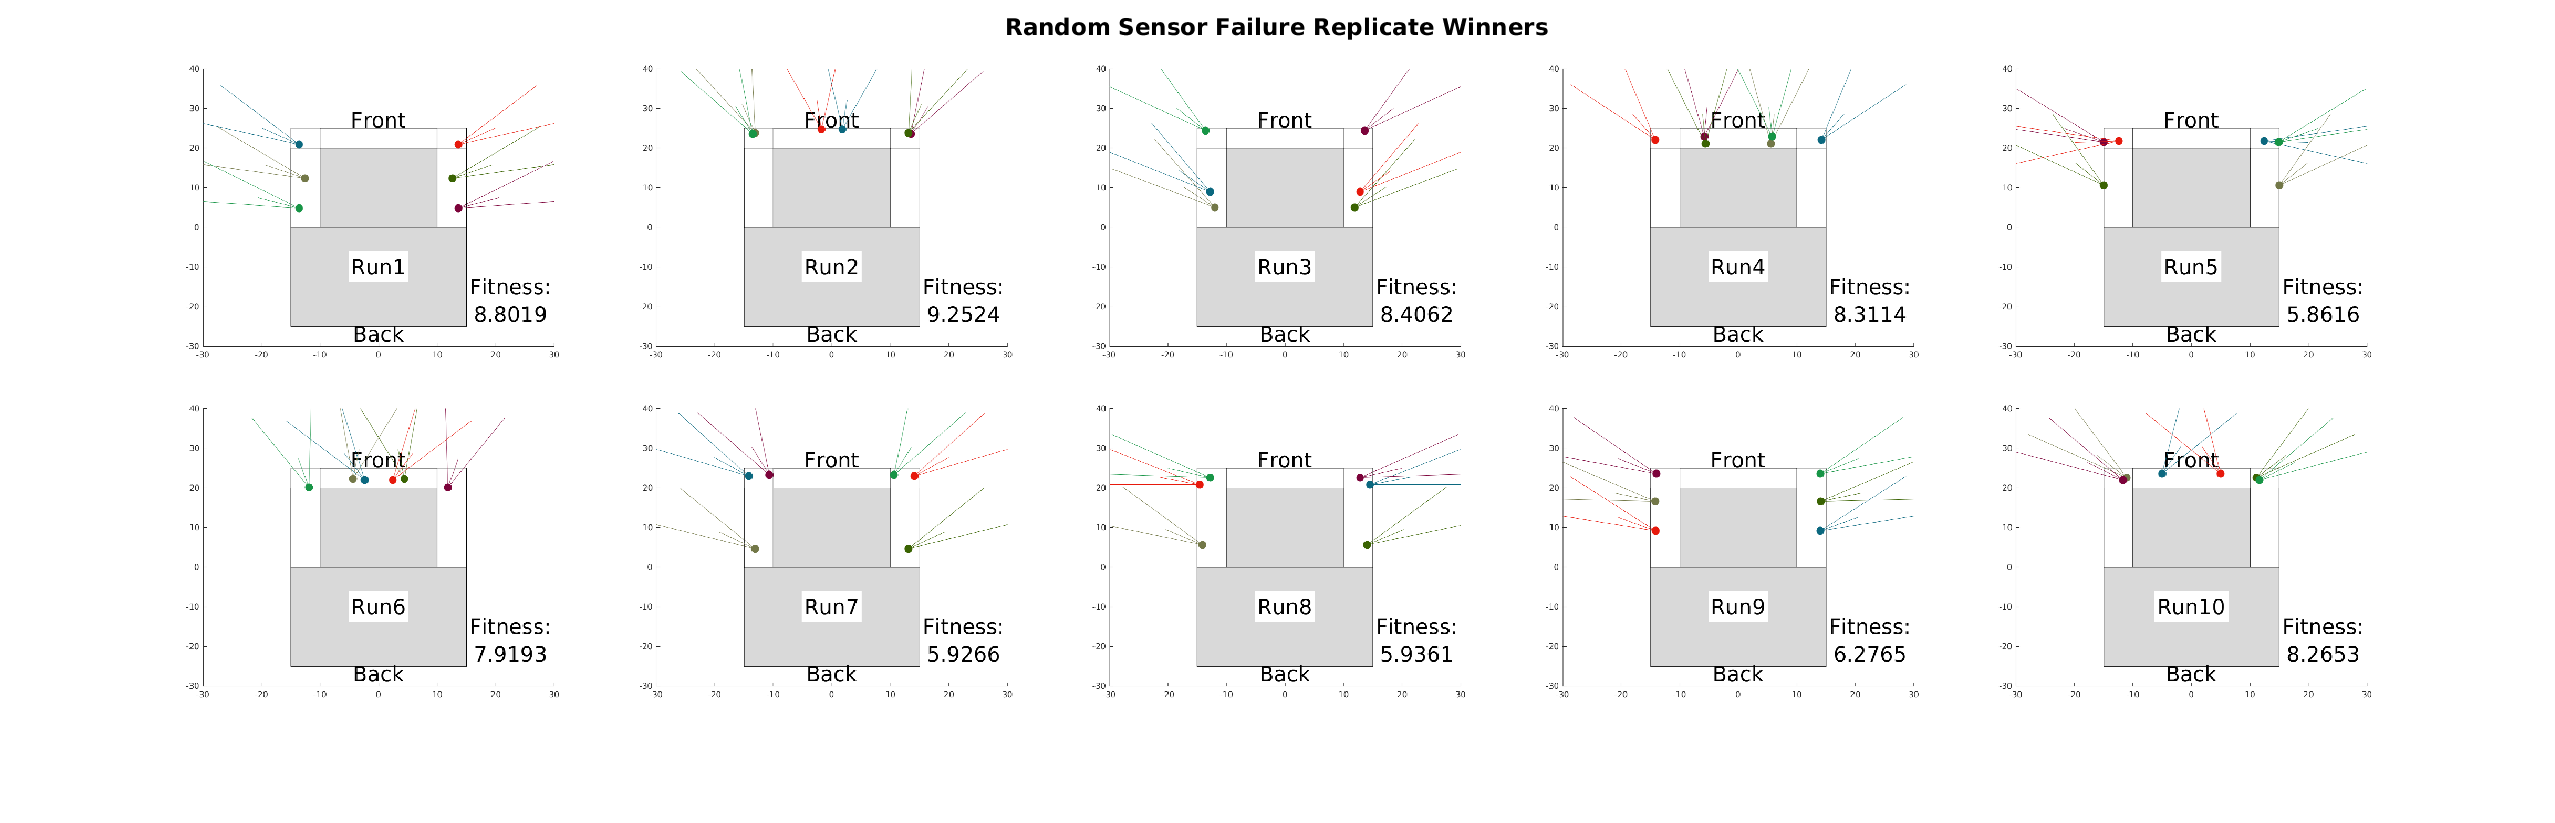
\includegraphics[width=0.95\textwidth]{Figures/6_sonar_symmetric_placement_with_complete_failure_winners_panel_2X5}
%     \caption{A panel image showing the winning sensor configuration for each replicate in the Random Failure Treatment.}
%     \label{random_failure_panel_fig}
% \end{figure*}

% \vspace{-0.1in}
\paragraph{Spatially Correlated Sensor Failure}

%This treatment explores the placement of sensors in situations where 
%sensor failures are correlated spatially, for example, due to physical
%damage in to an area of the vehicle.
%The configuration is is the same as in the previous treatment, with the 
%exception of the sensor failure model.
%In this treatment, at the start of each simulation a random time for failure is selected between 40 and 80 seconds, as was the case with the random failure scenario. However, now at the time of failure a random sensor is selected by the Sonar Filter process. This sensor is the considered to be the point of impact for the damage. From this sensor, three concentric circles are formed with radii of 3, 6, and 9cm, shown in figure \ref{spatial_failure_model}. Sensors within 3cm of the point of impact are guaranteed to fail. Sensors within 6 and 9cm have a 75 and 50\% chance of failing respectively. The Sonar Filter does not relay any data from a failed sensor and failed sensors do not have the chance to become active again for the duration of the mission.

Spatially correlated sensor failure simulates physical damage to a robot.  
%
Figure~\ref{spatial_failure_model} depicts
the spatial failure model centered on a sensor selected at random.  
%
Sensors within the affected area are also damaged and stop reporting.  
%
We hypothesize that this will pressure the sensors to be more evenly distributed across the robot and perhaps also demonstrate redundancy of coverage among the six sensors.  



\begin{figure}[ht]
%	\vspace{-0.1in}
	\centering
    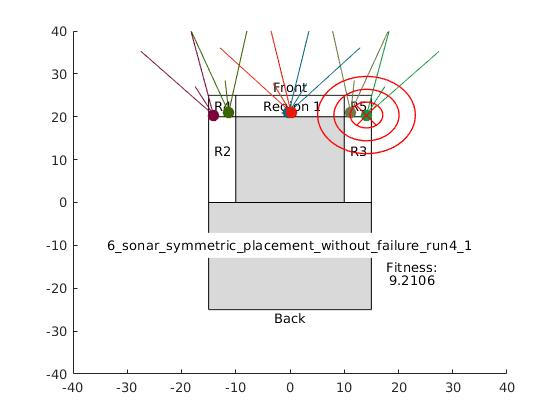
\includegraphics[width=0.4\textwidth]{Figures/6_sonar_failure_model.jpg}
    \vspace{-0.15in}
    \caption{The areas impacted by the spatially correlated failure model on a sample sensor configuration.}
    \label{spatial_failure_model}
%    \vspace{-0.15in}
\end{figure}

Figure~\ref{spatial_failure_panel_fig} plots the sensor placement of the highest performing individual in each of the ten replicates.
%
As in the baseline treatment, two primary configurations evolve.
%
The first remains an even spread of sensors across the front face of the rover.  
%
The second is focused on the sides of the platform.  
%
Surprisingly, there are clusters of sensors that would fall within the failure radius of the model.  
%
Apparently, the position of these sensors is more important than the risk of damage from sensor failures.    

% \begin{figure}[ht]
% 	\centering
%     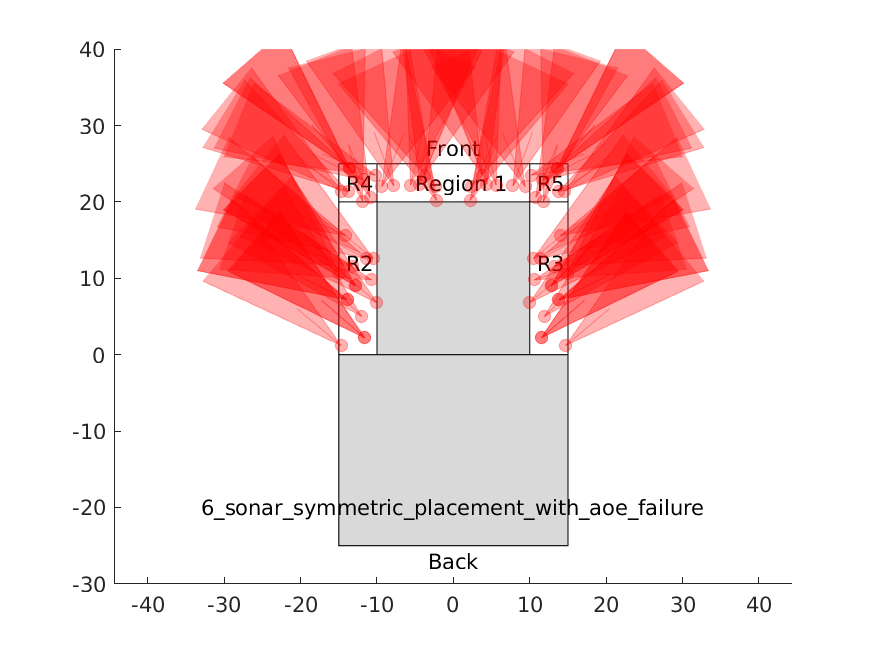
\includegraphics[width=0.4\textwidth]{Figures/6_sonar_symmetric_placement_with_aoe_failure_sensor_viewing_area_overlay.png}
%     \caption{Overlay of sensor placements and viewing areas from 10 replicates of the spatially correlated failure treatment experiment.}
%     \label{spatial_failure_overlay_fig}
% \end{figure}


\begin{figure*}[!htb]
	\centering
    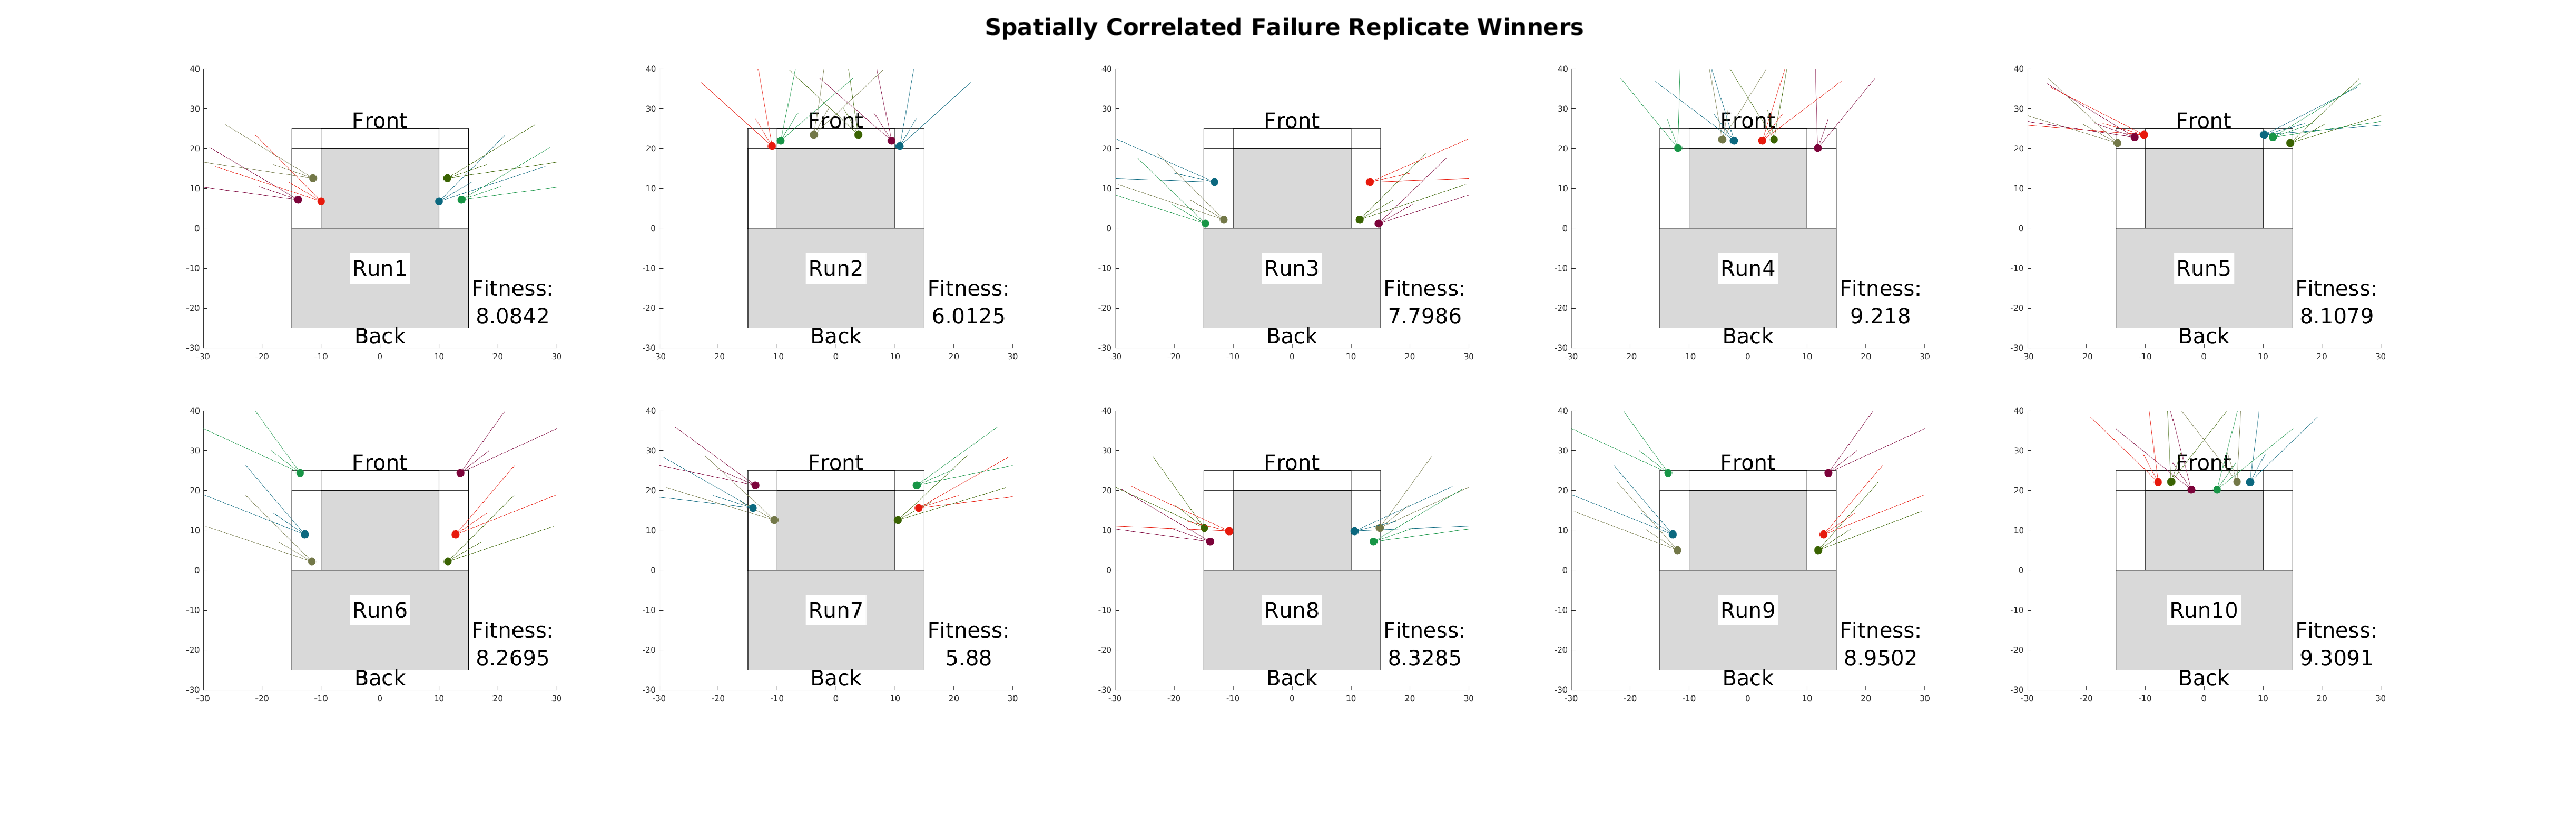
\includegraphics[width=0.95\textwidth]{Figures/6_sonar_symmetric_placement_with_aoe_failure_winners_panel_2x5.png}
    \vspace{-0.3in}
    \caption{A panel image showing winning sensor configuration for each replicate with spatially correlated failures.}
    \label{spatial_failure_panel_fig}
%    \vspace{-0.2in}
\end{figure*}





\section{Conclusions and Future Directions}
\label{s:conclusions}

%%%%%%%%%%%%%%%%%%%%%%%%%%%%%%%%
% Evo-ROS
Evo-ROS is intended as a bridge between the ER and traditional robotics communities.  
%
Leveraging the ROS/Gazebo simulation stack, evolutionary optimization can be applied to simulated robotic systems with pre-built and tested models of commercially available hardware.  
%
This approach should reduce developer time requirements in building an accurate simulation, and also increase the scope of available environments/platforms for the ER community.  
To address the execution time needed for high-fidelity simulations,
Evo-ROS provides an interface to parallelize evolutionary runs across multiple VMs.%

In a case study, we investigated optimization of sensor placement on the Erle-Rover, a commercially available UGV, equipped with with pre-built sensor libraries provided by ROS/Gazebo.  
Evolved solutions exhibit both expected~(front facing) and unexpected~(side facing) sensor deployments.  
%
% However, effective solutions evolve across the three treatments.  
%
Resilience to damage is an important need in robotic systems, but can be challenging to design into a system.  
%
Even in the presence of sensor failure, evolved solutions are able to complete the waypoint following tasks.  
%
Evolutionary search explores the possible space and can potentially suggest novel solutions to address this issue, as observed in this study.
%%%%%%%%%%%%%%%%%%%%%%%%%%%%%%%%

%%%%%%%%%%%%%%%%%%%%%%%%%%%%%%%%
% Evo-ROS is intended as a bridge between the ER and traditional robotics communities.  
%
% Leveraging the ROS/Gazebo simulation stack, evolutionary optimization can be applied to simulated robotic systems with pre-built and tested models of commercially available hardware.  
%
%This approach should reduce developer time requirements in building an accurate simulation, and also increase the scope of available environments/platforms for the ER community.  
%
%To address the execution time needed for high-fidelity simulations,
%Evo-ROS provides an interface to parallelize evolutionary runs across multiple VMs.  

While conducting the case study, we identified three areas for improvement/ongoing development.
First the Ardupilot control software employed on the rover limits the speed of simulations to real time.  
%
While Ardupilot-controlled commercial platforms are readily available, this controller is
intended primarily for the hobbyist market.  
%
In ongoing work, we are removing Ardupilot from the control stack of the rover, and will instead utilize a purely ROS-based controller.  
%
Doing so enables faster simulations and 
should not limit the available software stacks for control and sensing, 
as many other ROS/Gazebo software libraries are available. 
%%%%%%%%%%%%%%%%%%%%%%%%%%%%%%%%

%%%%%%%%%%%%%%%%%%%%%%%%%%%%%%%%
Second, the use of Ardupilot and its associated MAVProxy component limited our initial experiment to a single robot per environment.
%
Large-scale robotics problems might involve many robots per simulation.  
%
%
Our ongoing work eliminates the Ardupilot/MAVProxy dependency, allowing Evo-ROS to be used with
simulations containing multiple robotic agents.
%%%%%%%%%%%%%%%%%%%%%%%%%%%%%%%%

%%%%%%%%%%%%%%%%%%%%%%%%%%%%%%%%
% McKinley: Make more clear that we are building a VM not just a virtual environment.  
% How somebody can use it.  
% Everything is installed and ready to go.  
% Run as a VM on their system, or multiple instances of it.
Finally, the ROS/Gazebo software stack can have a high initial investment in terms of start-up and configuration.  
%
We are currently assembling a virtual machine, preconfigured with Evo-ROS and corresponding tutorials,
greatly reducing the time for new users to install and use Evo-ROS.
%
Rather than requiring individual installation of the many needed software packages, the 
VM will contain all necessary software, ready to run.  
%
A user can download and deploy a VM on their own system, or distribute many instances across a computing cluster and begin parallelized runs immediately.  
%
By eliminating many of the time-consuming challenges we encountered in developing Evo-ROS, we hope to facilitate
use of Evo-ROS by both the ER and mainstream robotics communities.


% % 1) This work combines evolutionary search with control software and simulation tools widely used by the mainstream robotics community through the use of Evo-ROS.

% % 2) Demonstrate the use of evolution to help design more resilient autonomous systems.
% % 2a) Apply evolution to determine the location of sonar sensors for waypoint following and obstacle avoidance in a commercial UGV, despite random sensor failures and physical damage affecting multiple sensors.

% %%%%%%%%%%%%%%%%%%%%%%%%%%%%%%%%
% % Sensor failure and resilience


% In this study, we investigated the optimization of sensor placement, taking
% into account possible failures, on a commercial UGV.
% % 5 tion of sonar sensor failure and its effect on a UGV based on the Erle-rover.  
% %
% Evolved solutions exhibit both expected~(front facing) and unexpected~(side facing) sensor deployments.  
% %
% % However, effective solutions evolve across the three treatments.  
% %
% Resilience to damage is an important need in robotic systems, but can be challenging to design into a system.  
% %
% Even in the presence of sensor failure, evolved solutions are able to complete the waypoint following tasks.  
% %
% Evolutionary search explores the possible space and can potentially suggest novel solutions to address this issue, as observed in this study.
% %%%%%%%%%%%%%%%%%%%%%%%%%%%%%%%%



% %%%%%%%%%%%%%%%%%%%%%%%%%%%%%%%%
% % Future Work
% In ongoing work, we plan to~(1) transfer these results to our physical rover for validation,~(2) improve the efficiency of the simulation by writing a custom autopilot, and~(3) continue investigating resilience across different platforms, including commercial aerial vehicles.
% %
% By using Evo-ROS, specifically ROS/Gazebo, evolved results on a simulated platform should be readily transferable to a physical system, potentially helping to reduce the reality gap.  
% %
% % We are developing a physical Erle-rover and plan to begin testing these, and other evolved controllers, in the near future.  
% %

% %%%%%%%%%%%%%%%%%%%%%%%%%%%%%%%%

\xpkm{
1. summarize results of the paper and contributions\\
2. futurework : conduct experiments with real robot.
Use evo-ros to explore resilient design and behavior in
other platforms, such a aquatic robots and aerial drones
(well supported by ROS, Gazebo, Ardupilot)}

\section*{Acknowledgments}
This work was supported in part by grants from the U.S. National Science Foundation and the Air Force Research Laboratory.  Additional support was provided by Grand Valley State University.
\bibliographystyle{abbrv}
\bibliography{References/pubs2011-present,References/references,References/website_references}

\end{document}
